\chapter{Searching for astrophysical neutrinos: High Energy Starting Events}

\section{Event selection\label{sec:selection}}
\begingroup
\graphicspath{{results/HESE_Final_Paper/}}
\chapter{Searching for astrophysical neutrinos}

\section{Event selection\label{sec:selection}}
\begingroup
\graphicspath{{results/HESE_Final_Paper/}}
\chapter{Searching for astrophysical neutrinos}

\section{Event selection\label{sec:selection}}
\begingroup
\graphicspath{{results/HESE_Final_Paper/}}
\chapter{Searching for astrophysical neutrinos}

\section{Event selection\label{sec:selection}}
\begingroup
\graphicspath{{results/HESE_Final_Paper/}}
\input{results/HESE_Final_Paper/sections/detectorselection/selection}
\endgroup

\section{Reconstruction and simulation}
\begingroup
\graphicspath{{results/HESE_Final_Paper/}}
\input{results/HESE_Final_Paper/sections/reconstruction}
\endgroup

\section{Systematic uncertainties and statistical treatment\label{sec:uncertainties}}
\subsection{Detector systematic uncertainties\label{sec:detector_systematics}}
\begingroup
\graphicspath{{results/HESE_Final_Paper/}}
\input{results/HESE_Final_Paper/sections/uncertainties/systematics}
\endgroup

\subsection{Statistical treatment\label{sec:statistics}}
\begingroup
\graphicspath{{results/HESE_Final_Paper/}}
\input{results/HESE_Final_Paper/sections/uncertainties/statistics}
\endgroup

\endgroup

\section{Reconstruction and simulation}
\begingroup
\graphicspath{{results/HESE_Final_Paper/}}
\chapter{Event reconstruction and simulation}\label{chapter:reconstruction}
\begingroup
\graphicspath{{results/HESE_Final_Paper/}}
\input{results/HESE_Final_Paper/sections/reconstruction}
\endgroup
\endgroup

\section{Systematic uncertainties and statistical treatment\label{sec:uncertainties}}
\subsection{Detector systematic uncertainties\label{sec:detector_systematics}}
\begingroup
\graphicspath{{results/HESE_Final_Paper/}}
\input{results/HESE_Final_Paper/sections/uncertainties/systematics}
\endgroup

\subsection{Statistical treatment\label{sec:statistics}}
\begingroup
\graphicspath{{results/HESE_Final_Paper/}}
\chapter{Statistics}\label{chapter:statistics}

\section{Systematic uncertainties and statistical treatment\label{sec:uncertainties}}
\subsection{Detector systematic uncertainties\label{sec:detector_systematics}}
\begingroup
\graphicspath{{results/HESE_Final_Paper/}}
\input{results/HESE_Final_Paper/sections/uncertainties/systematics}
\endgroup

\subsection{Statistical treatment\label{sec:statistics}}
\begingroup
\graphicspath{{results/HESE_Final_Paper/}}
\input{results/HESE_Final_Paper/sections/uncertainties/statistics}
\endgroup

\section{Dealing with limited simulation samples\label{sec:limited_simulation}}
The contents of this section is reproduced here with minor modifications from a collaborative work with Carlos A. Argüelles, and Tianlu Yuan~\cite{Arguelles:2019izp}.

\begingroup
\graphicspath{{results/mcllh_paper/}}
\input{results/mcllh_paper/sections/introduction}
\endgroup

\subsection{The Poisson likelihood and previous work\label{sec:mc_intro}}
\begingroup
\graphicspath{{results/mcllh_paper/}}
\input{results/mcllh_paper/sections/previous_work/poisson}
\endgroup

\subsubsection{The Barlow-Beeston likelihood}
\begingroup
\graphicspath{{results/mcllh_paper/}}
\input{results/mcllh_paper/sections/previous_work/bb}
\endgroup

\subsubsection{Uncertainties in the large-sample limit}
\begingroup
\graphicspath{{results/mcllh_paper/}}
\input{results/mcllh_paper/sections/previous_work/chi2}
\endgroup

\subsection{Generalization of the Poisson likelihood\label{sec:generalization_poisson}}
\begingroup
\graphicspath{{results/mcllh_paper/}}
\input{results/mcllh_paper/sections/generalized_poisson/generalized_poisson}
\endgroup

\subsubsection{Derivation of $\like (\lambda|\vecw(\vectheta))$ for identical weights\label{sec:constructing}}
\begingroup
\graphicspath{{results/mcllh_paper/}}
\input{results/mcllh_paper/sections/generalized_poisson/identical_weights}
\endgroup

\subsubsection{Extension to arbitrary weights\label{sec:extending}}
\begingroup
\graphicspath{{results/mcllh_paper/}}
\input{results/mcllh_paper/sections/generalized_poisson/arbitrary_weights}
\endgroup

\subsubsection{The effective likelihood\label{sec:effective}}
\begingroup
\graphicspath{{results/mcllh_paper/}}
\input{results/mcllh_paper/sections/generalized_poisson/effective_likelihood}
\endgroup

\subsubsection{A family of likelihoods\label{sec:priors}}
\begingroup
\graphicspath{{results/mcllh_paper/}}
\input{results/mcllh_paper/sections/generalized_poisson/family}
\endgroup

\subsubsection{Convergence of the effective likelihood\label{sec:llhconvergence}}
\begingroup
\graphicspath{{results/mcllh_paper/}}
\input{results/mcllh_paper/sections/generalized_poisson/convergence}
\endgroup

\subsubsection{Behavior of the effective likelihood\label{sec:llhbehavior}}
\begingroup
\graphicspath{{results/mcllh_paper/}}
\input{results/mcllh_paper/sections/generalized_poisson/behavior}
\endgroup

\subsection{Example and performance\label{sec:example}}
\begingroup
\graphicspath{{results/mcllh_paper/}}
\input{results/mcllh_paper/sections/example/example}
\endgroup

\subsubsection{Point estimation\label{sec:pointestimation}}
\begingroup
\graphicspath{{results/mcllh_paper/}}
\input{results/mcllh_paper/sections/example/point_estimation}
\endgroup

\subsubsection{Coverage\label{sec:coverage}}
\begingroup
\graphicspath{{results/mcllh_paper/}}
\input{results/mcllh_paper/sections/example/coverage}
\endgroup

\subsubsection{Posterior distributions\label{sec:posterior}}
\begingroup
\graphicspath{{results/mcllh_paper/}}
\input{results/mcllh_paper/sections/example/posterior}
\endgroup

\subsubsection{Performance\label{sec:performance}}
\begingroup
\graphicspath{{results/mcllh_paper/}}
\input{results/mcllh_paper/sections/example/performance}
\endgroup

\subsection{Conclusion\label{sec:llhconclusion}}
\begingroup
\graphicspath{{results/mcllh_paper/}}
\input{results/mcllh_paper/sections/conclusion}
\endgroup

\subsection{Summary of likelihood formulas\label{sec:llhtable}}
\begingroup
\graphicspath{{results/mcllh_paper/}}
\input{results/mcllh_paper/appendices/formulas}
\endgroup
\FloatBarrier
\section{Frequentist confidence intervals with nuisance parameters and limited simulation}\label{sec:low_stats_confidence_intervals}

Frequentist and Bayesian techniques deal with different two different kinds of probability.
In frequentist statistics, the relevant probability is the frequency of the outcome of a repeatable experiment.
Under this framework the important concepts are parameter estimation, confidence intervals, and statistical tests.
In Bayesian statistics, the relevant probabilities come from the application of Bayes theorem which means we can define the probability density of parameters.
This definition of the parameter p.d.f. is applicable to the same problems parameter estimation, interval construction, and statistical tests but comes at the cost of defining ``prior belief'' about parameters.

In this section we will ignore the problem of statistical tests, instead focusing on the common features that underpin parameter estimation and interval construction.
Generally in parameter estimation and interval construction there are two sets of parameters, parameters of interest $\vec\theta$ and nuisance parameters $\vec\eta$.
Fundamentally there is no distinction between these two kinds of parameters.
The difference is only in which parameters we want to infer information about.

For both parameter estimation and interval construction the likelihood function is central.
The likelihood function reflects the plausibility of model parameters given observed data and is defined as $\like(\vec\theta, \vec\eta|\textrm{data}) = p(\textrm{data}|\vec\theta, \vec\eta)$.
Where $p(\textrm{data}|\vec\theta, \vec\eta)$ is the probability of the data given the model parameters.
A useful technique to eliminate nuisance parameters is the profile likelihood technique.
Dropping the explicit notational dependence on data, the profile likelihood function is defined as
\begin{linenomath*}
	\begin{equation}
	\tilde{\like}^\texttt{profile}(\vec\theta) = \max_{\vec\eta} \like(\vec\theta,\vec\eta),
	\label{eq:likelihood_profile}
	\end{equation}
\end{linenomath*}
where often the negative log of the function is maximized in place of the function for computational reasons.
The profile likelihood is then only a function of the parameters of interest.
Parameter estimation can be performed by maximizing the profile likelihood to obtain the ``best-fit'' parameters
\begin{linenomath*}
	\begin{equation}
	\hat{\vec\theta} = \argmax_{\vec\theta} \tilde{\like}^\texttt{profile}(\vec\theta).
	\label{eq:best_fit}
	\end{equation}
\end{linenomath*}
This best-fit point in the parameter space is a derived property of the likelihood function.
However, the same procedure can be performed with other functions to the same effect.
In general a minimization procedure is used, and we refer to these functions as ``test-statistics'' (TS).
A particularly useful TS is derived directly from the profile likelihood technique,
\begin{linenomath*}
	\begin{equation}
	\TS(\vec\theta) = -2\log{\left(\frac{\tilde{\like}^\texttt{profile}(\vec\theta)}{\tilde{\like}^\texttt{profile}(\hat{\vec\theta})}\right)}.
	\end{equation}
\end{linenomath*}
Using this TS to perform parameter estimation through minimization is mathematically equivalent to maximizing the likelihood, however, this form will prove to be uniquely useful for interval construction.

Since frequentist statistics deals with the frequency of outcomes from repeated experiments we can use the TS that results from repeated experiments to construct probabilities.
Consider for a moment a single point in the parameter space $\vec\theta_0$.
At this point in the parameter space there is a distribution of data that can be observed, and therefore a distribution of TS functions.
Instead of considering the distribution of TS functions originating from this point, we can simplify the picture by looking at the TS function only evaluated at this point $\TS(\vec\theta_0)$.
This gives us a distribution of TS values for this point in the parameter space that may look like~\reffig{fig:TS_dist}.
\begin{figure}
	\centering
	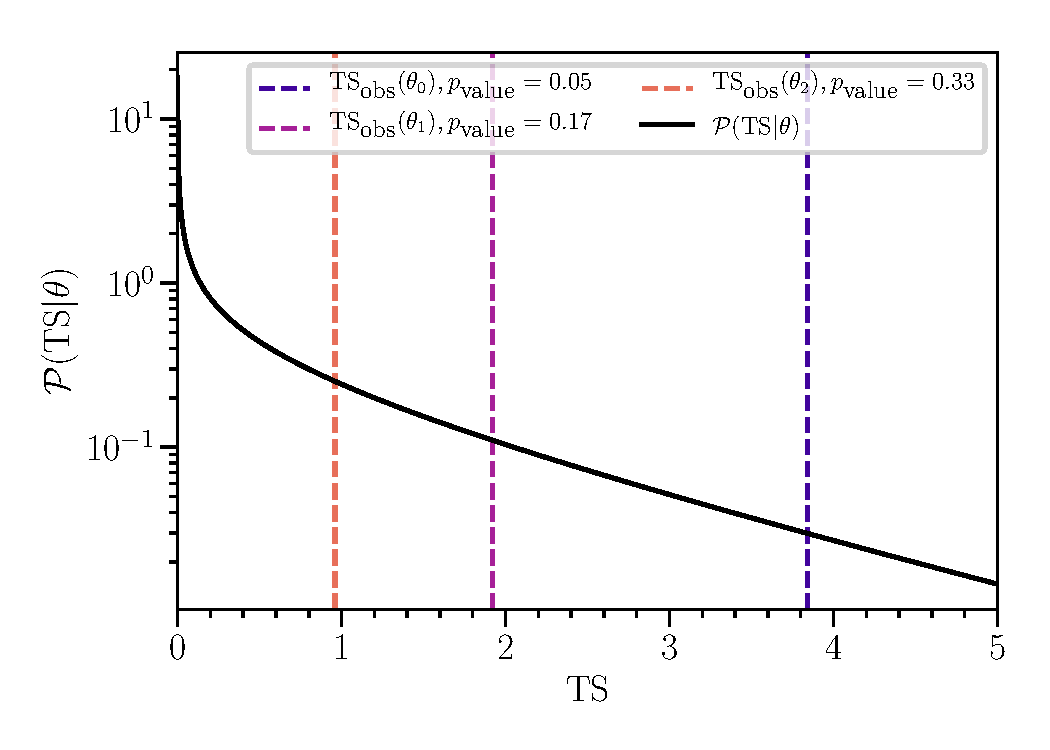
\includegraphics[width=0.8\linewidth]{figures/TS_dist}
	\caption{\textbf{\textit{Test statistic distribution.}} An example of a test statistic distribution.
	Such distributions tend to have the bulk of their mass close to the lower boundary with a long tail.
	Lower values indicate better statistical compatibility with the data.
	}
	\label{fig:TS_dist}
\end{figure}
It is important to note that for the profile likelihood TS and similar statistics a smaller TS value indicates better compatibility with the data.
For this reason many statistical tests are constructed using a single tail significance, by comparing the TS from a single experiment to a background TS distribution and reporting a p-value that is the fraction of the TS distribution greater than the observed TS.

This procedure can be extended to construct intervals by considering the TS distributions of every point in parameter space and comparing to the observed TS function.
Consider the one-dimensional case where there is a TS distribution for each value of the parameter, illustrated in~\reffig{fig:TS_dists_1d}
\begin{figure}
	\centering
	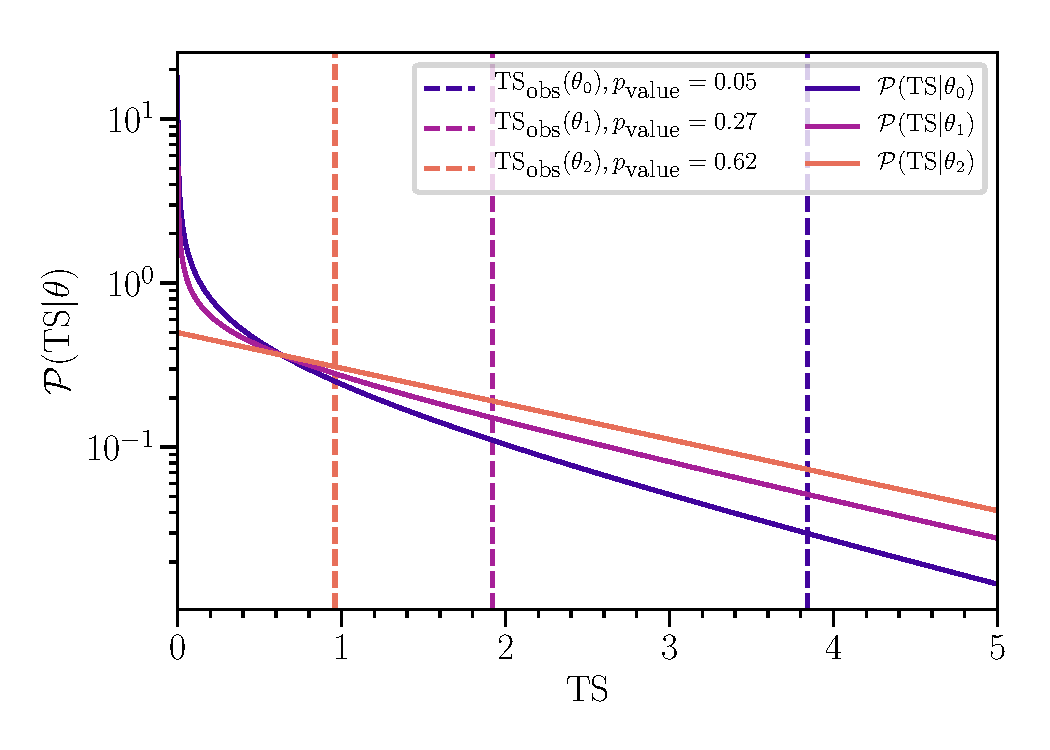
\includegraphics[width=0.8\linewidth]{figures/TS_dists_1d}
	\caption{\textbf{\textit{One-dimensional test-statistic distribution comparison.}} An example of the test statistic distributions as a function of a single parameter.
	}
	\label{fig:TS_dists_1d}
\end{figure}
We can construct an interval that will contain the true value of the parameter a fraction of the time $\alpha$ for repeated experiments.
This interval is the collection of points in the one-dimensional parameter space where the TS at that point is greater than the $\alpha$ quantile of the corresponding TS distribution.
If the TS distribution is the same for all points in parameter space, the interval construction can procedurally be thought of as drawing a horizontal line at the appropriate threshold and only including points that lie below the line.
Varying TS distributions modify this procedure to the comparison of two curves.
This procedure is not limited to one-dimension but can be extended to an arbitrary number of parameters of interest to construct n-dimensional regions with the same properties.

There is however an important caveat to this construction that appears when we consider nuisance parameters.
In order for the intervals to have the desired properties, the observed TS must be greater than the threshold for all possible values of the nuisance parameters.
This ultimatum presents several challenges.
Nuisance parameters can often have a broad or even unbounded range of allowed values, meaning if the effect of nuisance parameters does not taper off at the extrema then almost all intervals are guaranteed to be empty.
From a practical standpoint, computing the TS distributions for many points in parameter space is often done via Monte-Carlo and is computationally expensive.
Adding additional dimensions to the parameter space for which we must compute TS distributions exponentially increases the computation time.

To combat these issues we can limit our interval construction to be valid for values of the nuisance parameters that are ``reasonable''.
There are several methods for doing this, but we can split them into two categories: pure frequentist, and frequentist-Bayesian hybrid.
In the pure frequentist approaches we can either choose a single value of the nuisance parameters, or work with a limited range of the nuisance parameter values.
For the single value approach either nominal values are chosen before looking at the data, or estimators of the nuisance parameters are used to choose their values.
This approach benefits from simplicity, but fails if the test-statistic distributions vary rapidly with changes to the nuisance parameters for values that we might consider ``reasonable''.
A more expensive but robust approach is to explore the behavior of TS distributions for a limited range of the nuisance parameter values, which can be chosen {\it a priori} or from data-based bounds on the nuisance parameters.
If we are willing to consider a hybrid approach, then some more pragmatic options are available.

Although Bayesian methods could be used to choose a single point in parameter space from which to generate the TS distributions, the more interesting application is one that uses a distribution in parameter space.
In Bayesian statistics we can directly assign a probability density to the points in parameter space, either based on our prior information, or directly informed by the posterior distribution, from this extended perspective the probability of certain nuisance parameter values is of interest when considering the frequency of TS values for different parameters of interest.
The prior case is simple in that we sample the from the nuisance parameter priors when generating the TS distribution which allows us to account for variability introduced by the nuisance parameters without relying on hard cutoffs or biasing our inferences with parameter values that are unrealistic.
This prior based technique is well motivated if the priors are derived from external observations, however in the case where nuisance parameters have broad or ``uninformative'' priors this motivation and benefit may break down.
In some cases we expect nuisance parameters to be heavily constrained by the same data sample used to investigate the parameters of interest, so a different approach is merited.
The alternative is to use the posterior distribution to construct our nuisance parameter p.d.f.
Ideally a posterior distribution would be computed for each point in the parameters of interest space by fixing those parameters of interest.
In this way the nuisance parameter posterior used for sampling depends on the point in parameter space we are examining.

With the possible solutions available, we can now look at the problem of limited simulation size when generating test statistic distributions.
As explored in~\refsec{sec:limited_simulation} for binned Poisson likelihood problems, the real expectation in data or simulation for the number of events in a bin is not a known quantity.
Because the real expectations are not known, it is impossible to exactly model the distribution of TS that are expected for a particular point in the parameter space.
However, as~\refsec{sec:limited_simulation} also explored, limited simulation can be modeled with nuisance parameters so the techniques discussed above can be applied directly to the problem.
The ``single point in parameter space'' approach fails to address the additional uncertainty present in this case.
Allowing for unbounded variation of the bin expectations fails as it is guaranteed to produce empty intervals.
Bounding of the bin expectations within a reasonable range provides manageable intervals, but the dimensionality of the problem makes this computationally unfeasible beyond a handful of bins.
Unfortunately this excludes all the ``classic'' frequentist solutions to this problem.
The hybrid Bayesian-frequentist methods in this case provide a tractable solution that accounts for the additional uncertainty.
We can make use of the treatment described in~\refsec{sec:effective}, where the bin expectation is derived to be gamma distributed, and the expected number of data events modeled to be Poisson distributed once this expectation is known.
Practically this can be achieved by sampling data events from $\mcl$, or through a two step process where the expectation is sampled from a gamma distribution $\gprob(\lambda;\agpar, \bgpar)$ where $\agpar = \frac{\mu^2}{\sigma^2}+1~\textmd{and}~\bgpar=\frac{\mu}{\sigma^2}$, and the data events are sampled from a Poisson distribution $\frac{\lambda^{k}e^{-\lambda}}{k!}$.
It is important to note that this procedure only applies to variations in the data and should not be used to vary simulation expectations.
This is because the TS distribution is intended to model variations in the data, whereas the simulation used for analysis is fixed.
Combined with a similar hybrid treatment for other nuisance parameters, this provides a more complete accounting of the uncertainties given the available modeling.
\endgroup

\endgroup

\section{Reconstruction and simulation}
\begingroup
\graphicspath{{results/HESE_Final_Paper/}}
\chapter{Event reconstruction and simulation}\label{chapter:reconstruction}
\begingroup
\graphicspath{{results/HESE_Final_Paper/}}
\chapter{Event reconstruction and simulation}\label{chapter:reconstruction}
\begingroup
\graphicspath{{results/HESE_Final_Paper/}}
\input{results/HESE_Final_Paper/sections/reconstruction}
\endgroup
\endgroup
\endgroup

\section{Systematic uncertainties and statistical treatment\label{sec:uncertainties}}
\subsection{Detector systematic uncertainties\label{sec:detector_systematics}}
\begingroup
\graphicspath{{results/HESE_Final_Paper/}}
\input{results/HESE_Final_Paper/sections/uncertainties/systematics}
\endgroup

\subsection{Statistical treatment\label{sec:statistics}}
\begingroup
\graphicspath{{results/HESE_Final_Paper/}}
\chapter{Statistics}\label{chapter:statistics}

\section{Systematic uncertainties and statistical treatment\label{sec:uncertainties}}
\subsection{Detector systematic uncertainties\label{sec:detector_systematics}}
\begingroup
\graphicspath{{results/HESE_Final_Paper/}}
\input{results/HESE_Final_Paper/sections/uncertainties/systematics}
\endgroup

\subsection{Statistical treatment\label{sec:statistics}}
\begingroup
\graphicspath{{results/HESE_Final_Paper/}}
\chapter{Statistics}\label{chapter:statistics}

\section{Systematic uncertainties and statistical treatment\label{sec:uncertainties}}
\subsection{Detector systematic uncertainties\label{sec:detector_systematics}}
\begingroup
\graphicspath{{results/HESE_Final_Paper/}}
\input{results/HESE_Final_Paper/sections/uncertainties/systematics}
\endgroup

\subsection{Statistical treatment\label{sec:statistics}}
\begingroup
\graphicspath{{results/HESE_Final_Paper/}}
\input{results/HESE_Final_Paper/sections/uncertainties/statistics}
\endgroup

\section{Dealing with limited simulation samples\label{sec:limited_simulation}}
The contents of this section is reproduced here with minor modifications from a collaborative work with Carlos A. Argüelles, and Tianlu Yuan~\cite{Arguelles:2019izp}.

\begingroup
\graphicspath{{results/mcllh_paper/}}
\input{results/mcllh_paper/sections/introduction}
\endgroup

\subsection{The Poisson likelihood and previous work\label{sec:mc_intro}}
\begingroup
\graphicspath{{results/mcllh_paper/}}
\input{results/mcllh_paper/sections/previous_work/poisson}
\endgroup

\subsubsection{The Barlow-Beeston likelihood}
\begingroup
\graphicspath{{results/mcllh_paper/}}
\input{results/mcllh_paper/sections/previous_work/bb}
\endgroup

\subsubsection{Uncertainties in the large-sample limit}
\begingroup
\graphicspath{{results/mcllh_paper/}}
\input{results/mcllh_paper/sections/previous_work/chi2}
\endgroup

\subsection{Generalization of the Poisson likelihood\label{sec:generalization_poisson}}
\begingroup
\graphicspath{{results/mcllh_paper/}}
\input{results/mcllh_paper/sections/generalized_poisson/generalized_poisson}
\endgroup

\subsubsection{Derivation of $\like (\lambda|\vecw(\vectheta))$ for identical weights\label{sec:constructing}}
\begingroup
\graphicspath{{results/mcllh_paper/}}
\input{results/mcllh_paper/sections/generalized_poisson/identical_weights}
\endgroup

\subsubsection{Extension to arbitrary weights\label{sec:extending}}
\begingroup
\graphicspath{{results/mcllh_paper/}}
\input{results/mcllh_paper/sections/generalized_poisson/arbitrary_weights}
\endgroup

\subsubsection{The effective likelihood\label{sec:effective}}
\begingroup
\graphicspath{{results/mcllh_paper/}}
\input{results/mcllh_paper/sections/generalized_poisson/effective_likelihood}
\endgroup

\subsubsection{A family of likelihoods\label{sec:priors}}
\begingroup
\graphicspath{{results/mcllh_paper/}}
\input{results/mcllh_paper/sections/generalized_poisson/family}
\endgroup

\subsubsection{Convergence of the effective likelihood\label{sec:llhconvergence}}
\begingroup
\graphicspath{{results/mcllh_paper/}}
\input{results/mcllh_paper/sections/generalized_poisson/convergence}
\endgroup

\subsubsection{Behavior of the effective likelihood\label{sec:llhbehavior}}
\begingroup
\graphicspath{{results/mcllh_paper/}}
\input{results/mcllh_paper/sections/generalized_poisson/behavior}
\endgroup

\subsection{Example and performance\label{sec:example}}
\begingroup
\graphicspath{{results/mcllh_paper/}}
\input{results/mcllh_paper/sections/example/example}
\endgroup

\subsubsection{Point estimation\label{sec:pointestimation}}
\begingroup
\graphicspath{{results/mcllh_paper/}}
\input{results/mcllh_paper/sections/example/point_estimation}
\endgroup

\subsubsection{Coverage\label{sec:coverage}}
\begingroup
\graphicspath{{results/mcllh_paper/}}
\input{results/mcllh_paper/sections/example/coverage}
\endgroup

\subsubsection{Posterior distributions\label{sec:posterior}}
\begingroup
\graphicspath{{results/mcllh_paper/}}
\input{results/mcllh_paper/sections/example/posterior}
\endgroup

\subsubsection{Performance\label{sec:performance}}
\begingroup
\graphicspath{{results/mcllh_paper/}}
\input{results/mcllh_paper/sections/example/performance}
\endgroup

\subsection{Conclusion\label{sec:llhconclusion}}
\begingroup
\graphicspath{{results/mcllh_paper/}}
\input{results/mcllh_paper/sections/conclusion}
\endgroup

\subsection{Summary of likelihood formulas\label{sec:llhtable}}
\begingroup
\graphicspath{{results/mcllh_paper/}}
\input{results/mcllh_paper/appendices/formulas}
\endgroup
\FloatBarrier
\section{Frequentist confidence intervals with nuisance parameters and limited simulation}\label{sec:low_stats_confidence_intervals}

Frequentist and Bayesian techniques deal with different two different kinds of probability.
In frequentist statistics, the relevant probability is the frequency of the outcome of a repeatable experiment.
Under this framework the important concepts are parameter estimation, confidence intervals, and statistical tests.
In Bayesian statistics, the relevant probabilities come from the application of Bayes theorem which means we can define the probability density of parameters.
This definition of the parameter p.d.f. is applicable to the same problems parameter estimation, interval construction, and statistical tests but comes at the cost of defining ``prior belief'' about parameters.

In this section we will ignore the problem of statistical tests, instead focusing on the common features that underpin parameter estimation and interval construction.
Generally in parameter estimation and interval construction there are two sets of parameters, parameters of interest $\vec\theta$ and nuisance parameters $\vec\eta$.
Fundamentally there is no distinction between these two kinds of parameters.
The difference is only in which parameters we want to infer information about.

For both parameter estimation and interval construction the likelihood function is central.
The likelihood function reflects the plausibility of model parameters given observed data and is defined as $\like(\vec\theta, \vec\eta|\textrm{data}) = p(\textrm{data}|\vec\theta, \vec\eta)$.
Where $p(\textrm{data}|\vec\theta, \vec\eta)$ is the probability of the data given the model parameters.
A useful technique to eliminate nuisance parameters is the profile likelihood technique.
Dropping the explicit notational dependence on data, the profile likelihood function is defined as
\begin{linenomath*}
	\begin{equation}
	\tilde{\like}^\texttt{profile}(\vec\theta) = \max_{\vec\eta} \like(\vec\theta,\vec\eta),
	\label{eq:likelihood_profile}
	\end{equation}
\end{linenomath*}
where often the negative log of the function is maximized in place of the function for computational reasons.
The profile likelihood is then only a function of the parameters of interest.
Parameter estimation can be performed by maximizing the profile likelihood to obtain the ``best-fit'' parameters
\begin{linenomath*}
	\begin{equation}
	\hat{\vec\theta} = \argmax_{\vec\theta} \tilde{\like}^\texttt{profile}(\vec\theta).
	\label{eq:best_fit}
	\end{equation}
\end{linenomath*}
This best-fit point in the parameter space is a derived property of the likelihood function.
However, the same procedure can be performed with other functions to the same effect.
In general a minimization procedure is used, and we refer to these functions as ``test-statistics'' (TS).
A particularly useful TS is derived directly from the profile likelihood technique,
\begin{linenomath*}
	\begin{equation}
	\TS(\vec\theta) = -2\log{\left(\frac{\tilde{\like}^\texttt{profile}(\vec\theta)}{\tilde{\like}^\texttt{profile}(\hat{\vec\theta})}\right)}.
	\end{equation}
\end{linenomath*}
Using this TS to perform parameter estimation through minimization is mathematically equivalent to maximizing the likelihood, however, this form will prove to be uniquely useful for interval construction.

Since frequentist statistics deals with the frequency of outcomes from repeated experiments we can use the TS that results from repeated experiments to construct probabilities.
Consider for a moment a single point in the parameter space $\vec\theta_0$.
At this point in the parameter space there is a distribution of data that can be observed, and therefore a distribution of TS functions.
Instead of considering the distribution of TS functions originating from this point, we can simplify the picture by looking at the TS function only evaluated at this point $\TS(\vec\theta_0)$.
This gives us a distribution of TS values for this point in the parameter space that may look like~\reffig{fig:TS_dist}.
\begin{figure}
	\centering
	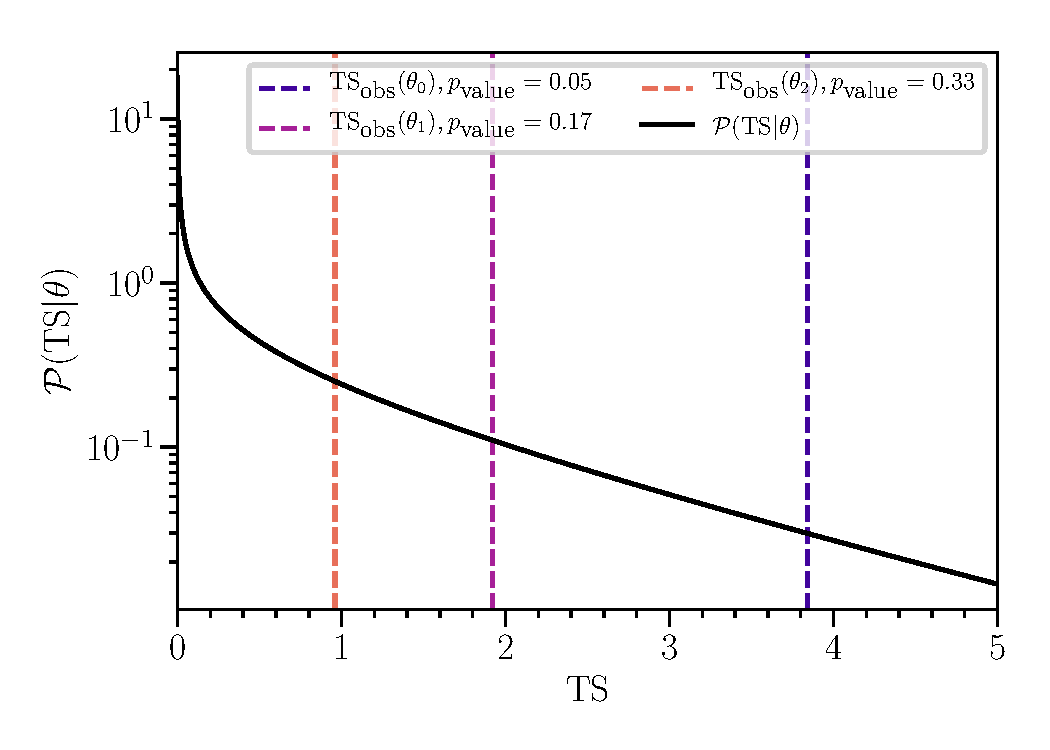
\includegraphics[width=0.8\linewidth]{figures/TS_dist}
	\caption{\textbf{\textit{Test statistic distribution.}} An example of a test statistic distribution.
	Such distributions tend to have the bulk of their mass close to the lower boundary with a long tail.
	Lower values indicate better statistical compatibility with the data.
	}
	\label{fig:TS_dist}
\end{figure}
It is important to note that for the profile likelihood TS and similar statistics a smaller TS value indicates better compatibility with the data.
For this reason many statistical tests are constructed using a single tail significance, by comparing the TS from a single experiment to a background TS distribution and reporting a p-value that is the fraction of the TS distribution greater than the observed TS.

This procedure can be extended to construct intervals by considering the TS distributions of every point in parameter space and comparing to the observed TS function.
Consider the one-dimensional case where there is a TS distribution for each value of the parameter, illustrated in~\reffig{fig:TS_dists_1d}
\begin{figure}
	\centering
	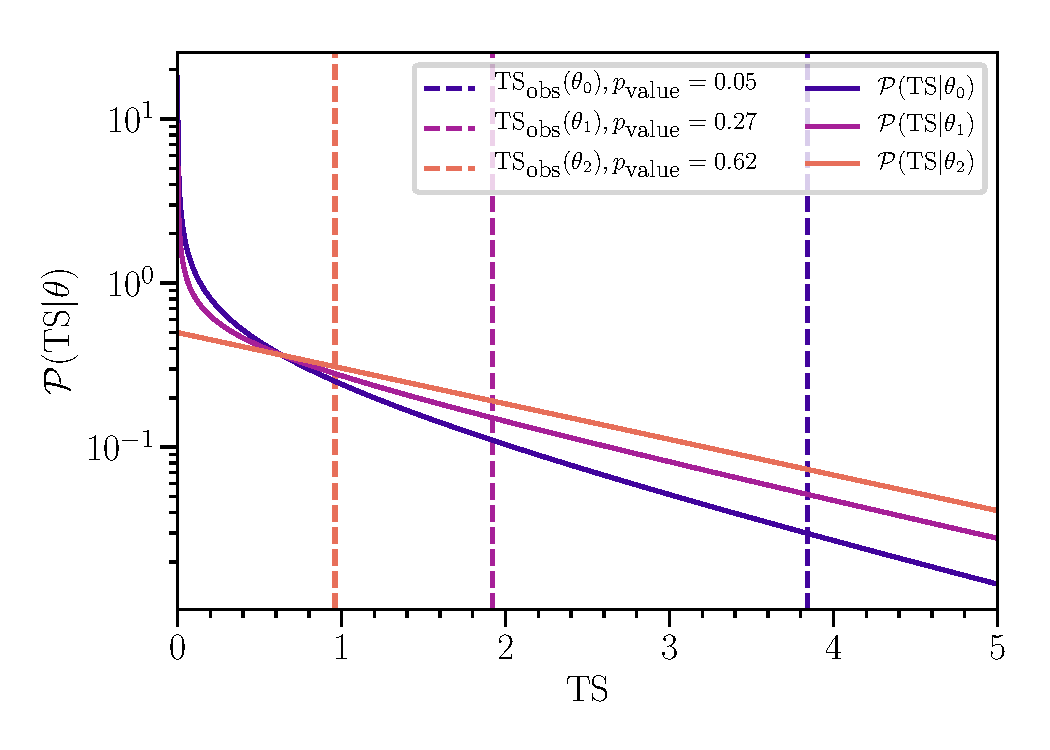
\includegraphics[width=0.8\linewidth]{figures/TS_dists_1d}
	\caption{\textbf{\textit{One-dimensional test-statistic distribution comparison.}} An example of the test statistic distributions as a function of a single parameter.
	}
	\label{fig:TS_dists_1d}
\end{figure}
We can construct an interval that will contain the true value of the parameter a fraction of the time $\alpha$ for repeated experiments.
This interval is the collection of points in the one-dimensional parameter space where the TS at that point is greater than the $\alpha$ quantile of the corresponding TS distribution.
If the TS distribution is the same for all points in parameter space, the interval construction can procedurally be thought of as drawing a horizontal line at the appropriate threshold and only including points that lie below the line.
Varying TS distributions modify this procedure to the comparison of two curves.
This procedure is not limited to one-dimension but can be extended to an arbitrary number of parameters of interest to construct n-dimensional regions with the same properties.

There is however an important caveat to this construction that appears when we consider nuisance parameters.
In order for the intervals to have the desired properties, the observed TS must be greater than the threshold for all possible values of the nuisance parameters.
This ultimatum presents several challenges.
Nuisance parameters can often have a broad or even unbounded range of allowed values, meaning if the effect of nuisance parameters does not taper off at the extrema then almost all intervals are guaranteed to be empty.
From a practical standpoint, computing the TS distributions for many points in parameter space is often done via Monte-Carlo and is computationally expensive.
Adding additional dimensions to the parameter space for which we must compute TS distributions exponentially increases the computation time.

To combat these issues we can limit our interval construction to be valid for values of the nuisance parameters that are ``reasonable''.
There are several methods for doing this, but we can split them into two categories: pure frequentist, and frequentist-Bayesian hybrid.
In the pure frequentist approaches we can either choose a single value of the nuisance parameters, or work with a limited range of the nuisance parameter values.
For the single value approach either nominal values are chosen before looking at the data, or estimators of the nuisance parameters are used to choose their values.
This approach benefits from simplicity, but fails if the test-statistic distributions vary rapidly with changes to the nuisance parameters for values that we might consider ``reasonable''.
A more expensive but robust approach is to explore the behavior of TS distributions for a limited range of the nuisance parameter values, which can be chosen {\it a priori} or from data-based bounds on the nuisance parameters.
If we are willing to consider a hybrid approach, then some more pragmatic options are available.

Although Bayesian methods could be used to choose a single point in parameter space from which to generate the TS distributions, the more interesting application is one that uses a distribution in parameter space.
In Bayesian statistics we can directly assign a probability density to the points in parameter space, either based on our prior information, or directly informed by the posterior distribution, from this extended perspective the probability of certain nuisance parameter values is of interest when considering the frequency of TS values for different parameters of interest.
The prior case is simple in that we sample the from the nuisance parameter priors when generating the TS distribution which allows us to account for variability introduced by the nuisance parameters without relying on hard cutoffs or biasing our inferences with parameter values that are unrealistic.
This prior based technique is well motivated if the priors are derived from external observations, however in the case where nuisance parameters have broad or ``uninformative'' priors this motivation and benefit may break down.
In some cases we expect nuisance parameters to be heavily constrained by the same data sample used to investigate the parameters of interest, so a different approach is merited.
The alternative is to use the posterior distribution to construct our nuisance parameter p.d.f.
Ideally a posterior distribution would be computed for each point in the parameters of interest space by fixing those parameters of interest.
In this way the nuisance parameter posterior used for sampling depends on the point in parameter space we are examining.

With the possible solutions available, we can now look at the problem of limited simulation size when generating test statistic distributions.
As explored in~\refsec{sec:limited_simulation} for binned Poisson likelihood problems, the real expectation in data or simulation for the number of events in a bin is not a known quantity.
Because the real expectations are not known, it is impossible to exactly model the distribution of TS that are expected for a particular point in the parameter space.
However, as~\refsec{sec:limited_simulation} also explored, limited simulation can be modeled with nuisance parameters so the techniques discussed above can be applied directly to the problem.
The ``single point in parameter space'' approach fails to address the additional uncertainty present in this case.
Allowing for unbounded variation of the bin expectations fails as it is guaranteed to produce empty intervals.
Bounding of the bin expectations within a reasonable range provides manageable intervals, but the dimensionality of the problem makes this computationally unfeasible beyond a handful of bins.
Unfortunately this excludes all the ``classic'' frequentist solutions to this problem.
The hybrid Bayesian-frequentist methods in this case provide a tractable solution that accounts for the additional uncertainty.
We can make use of the treatment described in~\refsec{sec:effective}, where the bin expectation is derived to be gamma distributed, and the expected number of data events modeled to be Poisson distributed once this expectation is known.
Practically this can be achieved by sampling data events from $\mcl$, or through a two step process where the expectation is sampled from a gamma distribution $\gprob(\lambda;\agpar, \bgpar)$ where $\agpar = \frac{\mu^2}{\sigma^2}+1~\textmd{and}~\bgpar=\frac{\mu}{\sigma^2}$, and the data events are sampled from a Poisson distribution $\frac{\lambda^{k}e^{-\lambda}}{k!}$.
It is important to note that this procedure only applies to variations in the data and should not be used to vary simulation expectations.
This is because the TS distribution is intended to model variations in the data, whereas the simulation used for analysis is fixed.
Combined with a similar hybrid treatment for other nuisance parameters, this provides a more complete accounting of the uncertainties given the available modeling.
\endgroup

\section{Dealing with limited simulation samples\label{sec:limited_simulation}}
The contents of this section is reproduced here with minor modifications from a collaborative work with Carlos A. Argüelles, and Tianlu Yuan~\cite{Arguelles:2019izp}.

\begingroup
\graphicspath{{results/mcllh_paper/}}
\chapter{Introduction}


\endgroup

\subsection{The Poisson likelihood and previous work\label{sec:mc_intro}}
\begingroup
\graphicspath{{results/mcllh_paper/}}
\input{results/mcllh_paper/sections/previous_work/poisson}
\endgroup

\subsubsection{The Barlow-Beeston likelihood}
\begingroup
\graphicspath{{results/mcllh_paper/}}
\input{results/mcllh_paper/sections/previous_work/bb}
\endgroup

\subsubsection{Uncertainties in the large-sample limit}
\begingroup
\graphicspath{{results/mcllh_paper/}}
\input{results/mcllh_paper/sections/previous_work/chi2}
\endgroup

\subsection{Generalization of the Poisson likelihood\label{sec:generalization_poisson}}
\begingroup
\graphicspath{{results/mcllh_paper/}}
\input{results/mcllh_paper/sections/generalized_poisson/generalized_poisson}
\endgroup

\subsubsection{Derivation of $\like (\lambda|\vecw(\vectheta))$ for identical weights\label{sec:constructing}}
\begingroup
\graphicspath{{results/mcllh_paper/}}
\input{results/mcllh_paper/sections/generalized_poisson/identical_weights}
\endgroup

\subsubsection{Extension to arbitrary weights\label{sec:extending}}
\begingroup
\graphicspath{{results/mcllh_paper/}}
\input{results/mcllh_paper/sections/generalized_poisson/arbitrary_weights}
\endgroup

\subsubsection{The effective likelihood\label{sec:effective}}
\begingroup
\graphicspath{{results/mcllh_paper/}}
\input{results/mcllh_paper/sections/generalized_poisson/effective_likelihood}
\endgroup

\subsubsection{A family of likelihoods\label{sec:priors}}
\begingroup
\graphicspath{{results/mcllh_paper/}}
\input{results/mcllh_paper/sections/generalized_poisson/family}
\endgroup

\subsubsection{Convergence of the effective likelihood\label{sec:llhconvergence}}
\begingroup
\graphicspath{{results/mcllh_paper/}}
\input{results/mcllh_paper/sections/generalized_poisson/convergence}
\endgroup

\subsubsection{Behavior of the effective likelihood\label{sec:llhbehavior}}
\begingroup
\graphicspath{{results/mcllh_paper/}}
\input{results/mcllh_paper/sections/generalized_poisson/behavior}
\endgroup

\subsection{Example and performance\label{sec:example}}
\begingroup
\graphicspath{{results/mcllh_paper/}}
\input{results/mcllh_paper/sections/example/example}
\endgroup

\subsubsection{Point estimation\label{sec:pointestimation}}
\begingroup
\graphicspath{{results/mcllh_paper/}}
\input{results/mcllh_paper/sections/example/point_estimation}
\endgroup

\subsubsection{Coverage\label{sec:coverage}}
\begingroup
\graphicspath{{results/mcllh_paper/}}
\input{results/mcllh_paper/sections/example/coverage}
\endgroup

\subsubsection{Posterior distributions\label{sec:posterior}}
\begingroup
\graphicspath{{results/mcllh_paper/}}
\input{results/mcllh_paper/sections/example/posterior}
\endgroup

\subsubsection{Performance\label{sec:performance}}
\begingroup
\graphicspath{{results/mcllh_paper/}}
\input{results/mcllh_paper/sections/example/performance}
\endgroup

\subsection{Conclusion\label{sec:llhconclusion}}
\begingroup
\graphicspath{{results/mcllh_paper/}}
\input{results/mcllh_paper/sections/conclusion}
\endgroup

\subsection{Summary of likelihood formulas\label{sec:llhtable}}
\begingroup
\graphicspath{{results/mcllh_paper/}}
\input{results/mcllh_paper/appendices/formulas}
\endgroup
\FloatBarrier
\section{Frequentist confidence intervals with nuisance parameters and limited simulation}\label{sec:low_stats_confidence_intervals}

Frequentist and Bayesian techniques deal with different two different kinds of probability.
In frequentist statistics, the relevant probability is the frequency of the outcome of a repeatable experiment.
Under this framework the important concepts are parameter estimation, confidence intervals, and statistical tests.
In Bayesian statistics, the relevant probabilities come from the application of Bayes theorem which means we can define the probability density of parameters.
This definition of the parameter p.d.f. is applicable to the same problems parameter estimation, interval construction, and statistical tests but comes at the cost of defining ``prior belief'' about parameters.

In this section we will ignore the problem of statistical tests, instead focusing on the common features that underpin parameter estimation and interval construction.
Generally in parameter estimation and interval construction there are two sets of parameters, parameters of interest $\vec\theta$ and nuisance parameters $\vec\eta$.
Fundamentally there is no distinction between these two kinds of parameters.
The difference is only in which parameters we want to infer information about.

For both parameter estimation and interval construction the likelihood function is central.
The likelihood function reflects the plausibility of model parameters given observed data and is defined as $\like(\vec\theta, \vec\eta|\textrm{data}) = p(\textrm{data}|\vec\theta, \vec\eta)$.
Where $p(\textrm{data}|\vec\theta, \vec\eta)$ is the probability of the data given the model parameters.
A useful technique to eliminate nuisance parameters is the profile likelihood technique.
Dropping the explicit notational dependence on data, the profile likelihood function is defined as
\begin{linenomath*}
	\begin{equation}
	\tilde{\like}^\texttt{profile}(\vec\theta) = \max_{\vec\eta} \like(\vec\theta,\vec\eta),
	\label{eq:likelihood_profile}
	\end{equation}
\end{linenomath*}
where often the negative log of the function is maximized in place of the function for computational reasons.
The profile likelihood is then only a function of the parameters of interest.
Parameter estimation can be performed by maximizing the profile likelihood to obtain the ``best-fit'' parameters
\begin{linenomath*}
	\begin{equation}
	\hat{\vec\theta} = \argmax_{\vec\theta} \tilde{\like}^\texttt{profile}(\vec\theta).
	\label{eq:best_fit}
	\end{equation}
\end{linenomath*}
This best-fit point in the parameter space is a derived property of the likelihood function.
However, the same procedure can be performed with other functions to the same effect.
In general a minimization procedure is used, and we refer to these functions as ``test-statistics'' (TS).
A particularly useful TS is derived directly from the profile likelihood technique,
\begin{linenomath*}
	\begin{equation}
	\TS(\vec\theta) = -2\log{\left(\frac{\tilde{\like}^\texttt{profile}(\vec\theta)}{\tilde{\like}^\texttt{profile}(\hat{\vec\theta})}\right)}.
	\end{equation}
\end{linenomath*}
Using this TS to perform parameter estimation through minimization is mathematically equivalent to maximizing the likelihood, however, this form will prove to be uniquely useful for interval construction.

Since frequentist statistics deals with the frequency of outcomes from repeated experiments we can use the TS that results from repeated experiments to construct probabilities.
Consider for a moment a single point in the parameter space $\vec\theta_0$.
At this point in the parameter space there is a distribution of data that can be observed, and therefore a distribution of TS functions.
Instead of considering the distribution of TS functions originating from this point, we can simplify the picture by looking at the TS function only evaluated at this point $\TS(\vec\theta_0)$.
This gives us a distribution of TS values for this point in the parameter space that may look like~\reffig{fig:TS_dist}.
\begin{figure}
	\centering
	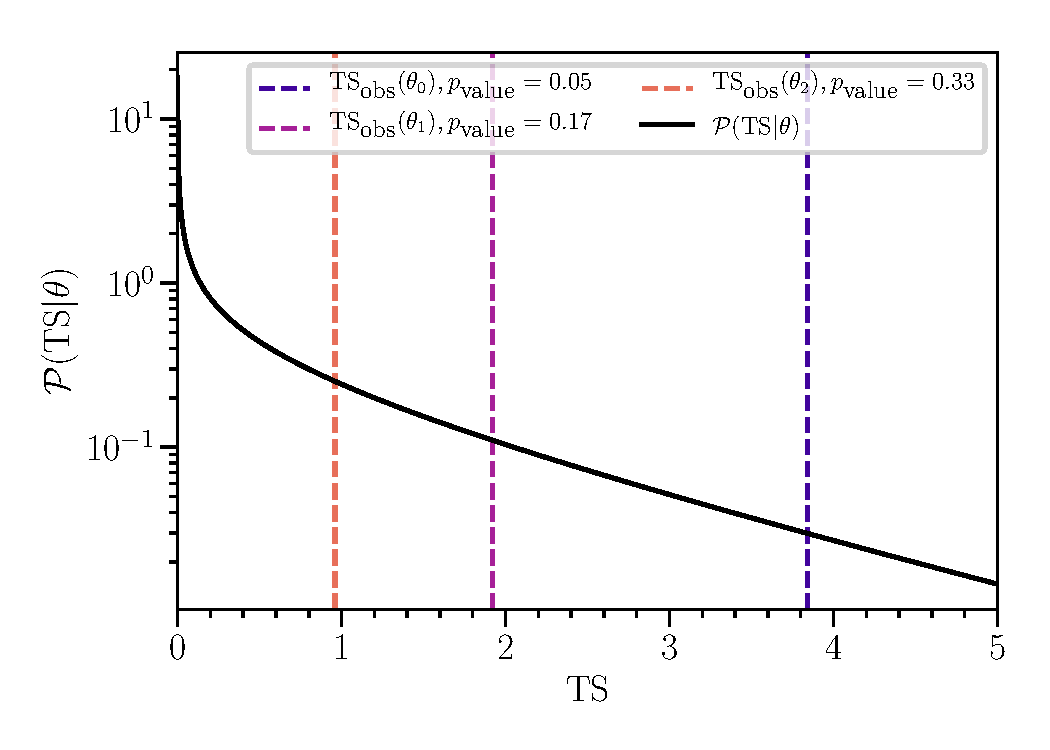
\includegraphics[width=0.8\linewidth]{figures/TS_dist}
	\caption{\textbf{\textit{Test statistic distribution.}} An example of a test statistic distribution.
	Such distributions tend to have the bulk of their mass close to the lower boundary with a long tail.
	Lower values indicate better statistical compatibility with the data.
	}
	\label{fig:TS_dist}
\end{figure}
It is important to note that for the profile likelihood TS and similar statistics a smaller TS value indicates better compatibility with the data.
For this reason many statistical tests are constructed using a single tail significance, by comparing the TS from a single experiment to a background TS distribution and reporting a p-value that is the fraction of the TS distribution greater than the observed TS.

This procedure can be extended to construct intervals by considering the TS distributions of every point in parameter space and comparing to the observed TS function.
Consider the one-dimensional case where there is a TS distribution for each value of the parameter, illustrated in~\reffig{fig:TS_dists_1d}
\begin{figure}
	\centering
	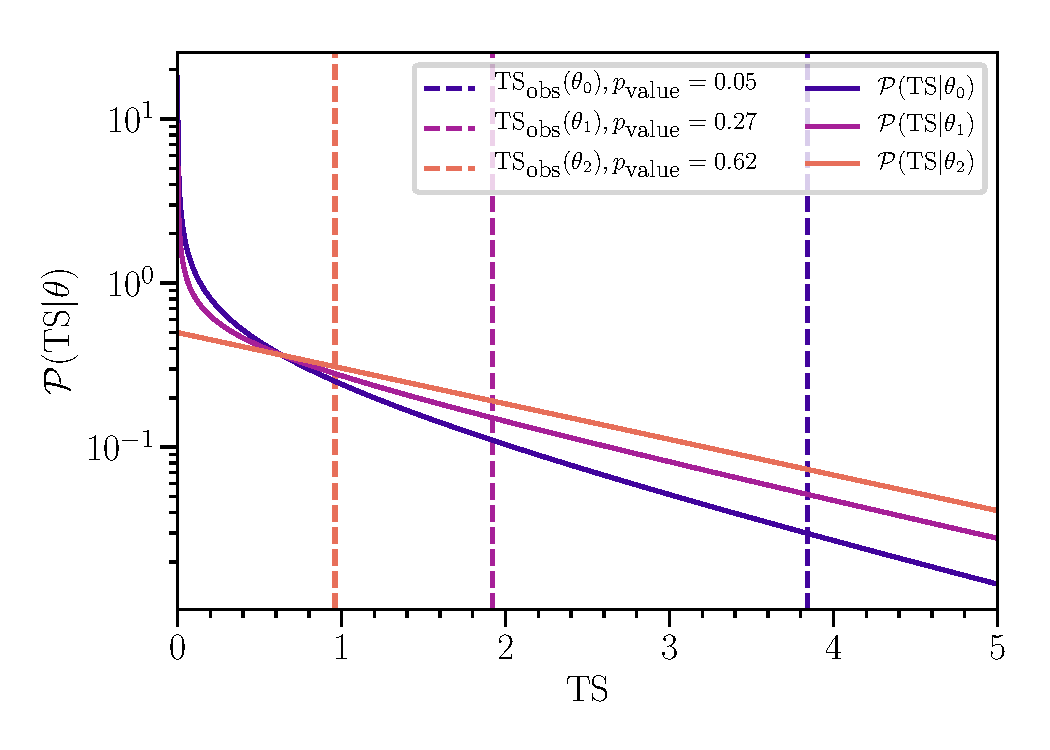
\includegraphics[width=0.8\linewidth]{figures/TS_dists_1d}
	\caption{\textbf{\textit{One-dimensional test-statistic distribution comparison.}} An example of the test statistic distributions as a function of a single parameter.
	}
	\label{fig:TS_dists_1d}
\end{figure}
We can construct an interval that will contain the true value of the parameter a fraction of the time $\alpha$ for repeated experiments.
This interval is the collection of points in the one-dimensional parameter space where the TS at that point is greater than the $\alpha$ quantile of the corresponding TS distribution.
If the TS distribution is the same for all points in parameter space, the interval construction can procedurally be thought of as drawing a horizontal line at the appropriate threshold and only including points that lie below the line.
Varying TS distributions modify this procedure to the comparison of two curves.
This procedure is not limited to one-dimension but can be extended to an arbitrary number of parameters of interest to construct n-dimensional regions with the same properties.

There is however an important caveat to this construction that appears when we consider nuisance parameters.
In order for the intervals to have the desired properties, the observed TS must be greater than the threshold for all possible values of the nuisance parameters.
This ultimatum presents several challenges.
Nuisance parameters can often have a broad or even unbounded range of allowed values, meaning if the effect of nuisance parameters does not taper off at the extrema then almost all intervals are guaranteed to be empty.
From a practical standpoint, computing the TS distributions for many points in parameter space is often done via Monte-Carlo and is computationally expensive.
Adding additional dimensions to the parameter space for which we must compute TS distributions exponentially increases the computation time.

To combat these issues we can limit our interval construction to be valid for values of the nuisance parameters that are ``reasonable''.
There are several methods for doing this, but we can split them into two categories: pure frequentist, and frequentist-Bayesian hybrid.
In the pure frequentist approaches we can either choose a single value of the nuisance parameters, or work with a limited range of the nuisance parameter values.
For the single value approach either nominal values are chosen before looking at the data, or estimators of the nuisance parameters are used to choose their values.
This approach benefits from simplicity, but fails if the test-statistic distributions vary rapidly with changes to the nuisance parameters for values that we might consider ``reasonable''.
A more expensive but robust approach is to explore the behavior of TS distributions for a limited range of the nuisance parameter values, which can be chosen {\it a priori} or from data-based bounds on the nuisance parameters.
If we are willing to consider a hybrid approach, then some more pragmatic options are available.

Although Bayesian methods could be used to choose a single point in parameter space from which to generate the TS distributions, the more interesting application is one that uses a distribution in parameter space.
In Bayesian statistics we can directly assign a probability density to the points in parameter space, either based on our prior information, or directly informed by the posterior distribution, from this extended perspective the probability of certain nuisance parameter values is of interest when considering the frequency of TS values for different parameters of interest.
The prior case is simple in that we sample the from the nuisance parameter priors when generating the TS distribution which allows us to account for variability introduced by the nuisance parameters without relying on hard cutoffs or biasing our inferences with parameter values that are unrealistic.
This prior based technique is well motivated if the priors are derived from external observations, however in the case where nuisance parameters have broad or ``uninformative'' priors this motivation and benefit may break down.
In some cases we expect nuisance parameters to be heavily constrained by the same data sample used to investigate the parameters of interest, so a different approach is merited.
The alternative is to use the posterior distribution to construct our nuisance parameter p.d.f.
Ideally a posterior distribution would be computed for each point in the parameters of interest space by fixing those parameters of interest.
In this way the nuisance parameter posterior used for sampling depends on the point in parameter space we are examining.

With the possible solutions available, we can now look at the problem of limited simulation size when generating test statistic distributions.
As explored in~\refsec{sec:limited_simulation} for binned Poisson likelihood problems, the real expectation in data or simulation for the number of events in a bin is not a known quantity.
Because the real expectations are not known, it is impossible to exactly model the distribution of TS that are expected for a particular point in the parameter space.
However, as~\refsec{sec:limited_simulation} also explored, limited simulation can be modeled with nuisance parameters so the techniques discussed above can be applied directly to the problem.
The ``single point in parameter space'' approach fails to address the additional uncertainty present in this case.
Allowing for unbounded variation of the bin expectations fails as it is guaranteed to produce empty intervals.
Bounding of the bin expectations within a reasonable range provides manageable intervals, but the dimensionality of the problem makes this computationally unfeasible beyond a handful of bins.
Unfortunately this excludes all the ``classic'' frequentist solutions to this problem.
The hybrid Bayesian-frequentist methods in this case provide a tractable solution that accounts for the additional uncertainty.
We can make use of the treatment described in~\refsec{sec:effective}, where the bin expectation is derived to be gamma distributed, and the expected number of data events modeled to be Poisson distributed once this expectation is known.
Practically this can be achieved by sampling data events from $\mcl$, or through a two step process where the expectation is sampled from a gamma distribution $\gprob(\lambda;\agpar, \bgpar)$ where $\agpar = \frac{\mu^2}{\sigma^2}+1~\textmd{and}~\bgpar=\frac{\mu}{\sigma^2}$, and the data events are sampled from a Poisson distribution $\frac{\lambda^{k}e^{-\lambda}}{k!}$.
It is important to note that this procedure only applies to variations in the data and should not be used to vary simulation expectations.
This is because the TS distribution is intended to model variations in the data, whereas the simulation used for analysis is fixed.
Combined with a similar hybrid treatment for other nuisance parameters, this provides a more complete accounting of the uncertainties given the available modeling.
\endgroup

\endgroup

\section{Estimation of backgrounds}

In the search for astrophysical neutrinos, the predominant backgrounds are from atmospheric neutrinos and atmospheric muons.
Single atmospheric neutrinos are able to produce the same event signatures as astrophysical neutrinos because they are not fundamentally different astrophysical neutrinos.
Atmospheric neutrinos can only be distinguished from their astrophysical counterparts by examining the population properties, or by the fact that muons produced in the same air shower can also reach the detector simultaneously.
Muons from cosmic ray air showers differ from neutrinos in their event signature as they always produce light while entering the detector, while neutrinos can interact within the detector volume before any light is produced near the edge of the detector.
Muons can also only be observed up to a certain amount of overburden, beyond which they will lose their energy and decay before reaching the detector.
This means the up-going observation region is free from atmospheric muons.

\subsection{Neutrino background estimation}

Atmospheric neutrinos are predominantly produced by the decay of pions and kaons, which we shall call the ``conventional'' component.
At energies above $\SI{1}\TeV$ the spectrum of the conventional component is softer than the incident cosmic-ray spectrum by one unit in the spectral index, due to the interactions of these mesons in the atmosphere.
The conventional neutrino flux is largest at the horizon, $\cos\theta_z=0$~\cite{Gaisser:2002jj,Barr:2004br,Honda:2006qj,Petrova:2012qf} because the larger path length in the thin atmosphere increases the proportion of pions that can decay before interacting.
To model the conventional neutrino flux, we use a parameterization of the Honda {\it{}et al.} 2006 flux calculation~\cite{Honda:2006qj} given in~\cite{Montaruli:2011as} which at the highest energies uses the analytic parameterization of the neutrino flux in~\cite{Gaisser:2002jj}.
This calculation is tuned to match observations of atmospheric muons, which remain difficult to predict from first principles.

A sub-leading -- yet unobserved -- contribution due to charmed hadron decays is expected to be important above $\sim\SI{100}\TeV$~\cite{Bhattacharya:2015jpa}.
Since the charmed hadrons decay promptly and do not interact in the atmosphere at the energies relevant for this analysis, we call this the ``prompt'' component.
Thus, at these energies, the prompt component has a spectral index close to the incident cosmic-ray spectrum.
The prompt flux is also constant with respect to the cosine of the zenith angle, as the short decay time of the charmed hadrons removes the effect of different path lengths through the atmosphere.
To model the prompt neutrino flux at Earth's surface, we use the flux computed in~\cite{Bhattacharya:2015jpa}.

The angular and energy distribution of the initial atmospheric neutrino flux is modified with respect to the flux at Earth's surface because of absorption of high-energy neutrinos in the Earth.
We account for this using a dedicated Monte Carlo, similar to the one described in~\cite{Gazizov:2004va}, that simulates the propagation of neutrinos in the Earth.
In this Monte Carlo we use the isoscalar neutrino cross sections given in~\cite{CooperSarkar:2011pa} for the neutrino-nucleon interactions, and the Earth density model described in~\cite{Dziewonski:1981xy}.
Neutrino-electron scattering can be safely neglected except for resonant-W production~\cite{Glashow:1960zz} which we include.
We ignore the uncertainties on the Earth opacity as they are known to be sub-leading in this energy range~\cite{Gandhi:1995tf,CooperSarkar:2011pa,Vincent:2017svp}.

Modeling the atmospheric neutrino flux with these two components does not account for the contribution of $K_s$~\cite{Gaisser:2014pda}, which is $\sim \SI{10}\percent$ at $\SI{100}\TeV$ and well-within our uncertainties.
In order to account for uncertainties in the cosmic-ray flux~\cite{Dembinski:2017zsh} and hadronic interactions~\cite{Fedynitch:2012fs} we parameterize the atmospheric neutrino flux as
\noindent
\begin{linenomath*}
	\begin{equation}
	\begin{split}
	\phi_\nu^{\rm{atm}} =& \Phi_{conv} \bigg(\phi^\pi_\nu + R_{K/\pi} \phi^K_\nu\bigg) {\bigg(\frac{E_\nu}{E_0^c} \bigg)}^{-\Delta \gamma_{CR}} \\ &+ \Phi_{prompt} \phi^p_\nu {\bigg(\frac{E_\nu}{E_0^p} \bigg)}^{-\Delta \gamma_{CR}},
	\end{split}
	\label{eq:atm_flux_equation}
	\end{equation}
\end{linenomath*}
where $\phi^\pi_\nu$, $\phi^K_\nu$, and $\phi^p_\nu$ are the conventional pion, kaon, and prompt atmospheric neutrino fluxes at a neutrino energy $E_\nu$ respectively.

The parameters $\convnorm$ and $\promptnorm$ are normalizations for the conventional and prompt normalizations respectively; $\pik$ allows us to modify the relative kaon to pion contributions; and the $\crdeltagamma$ parameter allows for hardening or softening of the atmospheric neutrino component to account for uncertainties in the cosmic-ray flux slope.
These parameters are incorporated into the analysis as nuisance parameters with priors as summarized in \reftab{tbl:priors}.
Priors are selected either to be Gaussian or uniform if otherwise unspecified.
This analysis refrains from directly using prior information from other IceCube neutrino studies in order to provide results independent from other samples.
The conventional normalization Gaussian prior width is motivated by studies of the total uncertainty due to cosmic-ray and high-energy hadronic processes~\cite{Fedynitch:2012fs}.
The width of the cosmic-ray slope parameter has been chosen to be $0.05$ in order to accommodate values measured at intermediate~\cite{Karelin:2011zz} and high~\cite{Bartoli:2015fhw,Yoon:2017qjx,Alfaro:2017cwx} energies.
The corrections to the ratios of neutrinos-to-anti-neutrinos and kaon-pion yields uncertainty was estimated by comparing the expectation of different atmospheric neutrino calculations and picking a width that encompasses their prediction.
Details regarding these corrections and the different atmospheric neutrino flux calculations can be found in~\cite{CollinFluxes,Jones:2015bya}.
Finally, the parameters $E_0^c=\SI{2020}\GeV$ and $E_0^p=\SI{7887}\GeV$ are points of fixed differential flux for the conventional and prompt components.

This simple parameterzation of the atmospheric neutrino flux and its uncertainties is chosen because it models the primary systematic effects of physical uncertainties that are observable with this sample.
Of course this neglects other physical uncertainties, such as those regarding the hadronic interactions in cosmic ray air showers and the composition of the cosmic ray particles.
But, these effects do not produce modifications to the observations that can be statistically discerned with the amount of data available.
Later it will be shown that even the modeled systematic uncertainties have a small effect on astrophysical measurements compared to the statistical uncertainties.

% Table of all systematics and their priors if applicable
\begin{table*}[thb]
	\centering
	% systematic parameter & prior type & mean & sigma & min & max
	\begin{tabular}{l rrr}
		%\toprule
		%& \multicolumn{5}{c}{Prior information} \\
		%\cmidrule{2-6}
		Parameter & Prior (constraint) & Range & Description \\
		\toprule
		\multicolumn{1}{l }{\textbf{Astrophysical neutrino flux:}} & & & \\
		$\astronorm$ & - & $[0,\infty)$ & Normalization scale\\
		$\astrodeltagamma$ & - &  $(-\infty,\infty)$ & Spectral index\\
		%$\theta_a$ & Uniform &  &  & 0 & 1 \\ \hline
		%$\theta_b$ & Uniform &  &  & -1 & 1 \\ \hline
		%${2\nu/\left(\nu+\bar{\nu}\right)}_\texttt{astro}$ & - & $[0,2]$\\
		&&\\
		\midrule
		\multicolumn{1}{l }{\textbf{Atmospheric neutrino flux:}} & & &\\
		$\convnorm$ & $1.0\pm0.4$ & $[0, \infty)$ & Conventional normalization scale\\
		$\promptnorm$ & - & $[0, \infty)$ & Prompt normalization scale\\
		$\pik$ & $1.0\pm0.1$ & $[0, \infty)$ & Kaon-Pion ratio correction\\
		$\atmonunubar$ & $1.0\pm0.1$ & $[0,2]$ & Neutrino-anti-neutrino ratio correction\\
		&&\\
		\midrule
		\multicolumn{1}{l }{\textbf{Cosmic ray flux:}} & & &\\
		$\crdeltagamma$ & $0.0\pm 0.05$ & $(-\infty,\infty)$ & Cosmic-ray spectral index modification\\
		$\muonnorm$ & $1.0\pm 0.5$ & $[0,\infty)$ & Muon normalization scale\\
		&&\\
		\midrule
		\multicolumn{1}{l }{\textbf{Detector:}} & & &\\
		$\domeff$ & $0.99 \pm 0.1$ & $[0.80, 1.25]$ & Absolute energy scale\\
		$\holeice$ & $0.0 \pm 0.5$ & $[-3.82, 2.18]$ & DOM angular response\\
		$\anisotropy$ & $1.0 \pm 0.2$ & $[0.0, 2.0]$ & Ice anisotropy scale\\
	\end{tabular}
	\internallinenumbers
	\caption{\textbf{\textit{Analysis model parameters for the single power-law astrophysical model.}} Prior probabilities (constraints) for analysis parameters used in Bayesian (frequentist) analyses respectively.
		Priors (constraints) on the parameter are either uniform or Gaussian.
		Where applicable, the mean, standard deviation, and bounds are given.}\label{tbl:priors}
\end{table*}


\subsection{Atmospheric neutrino passing fractions}

As noted in~\cite{Schonert:2008is}, muons produced in the same air-shower may trigger the detector veto in coincidence with the neutrino interaction.
Dedicated simulations of cosmic ray air showers where neutrino interactions are forced can provide observational predictions for the distribution of these combines muon+neutrino events.
However, available simulation techniques to create these estimates remain prohibitively expensive for the desired accuracy.
Instead, we look to model this effect by computing an average efficiency with respect to the case where no muons reach the detector.
To account for this when weighting the neutrino-only simulation each atmospheric neutrino flux component, $i$, is multiplied by an efficiency.
This efficiency is referred to as the ``atmospheric neutrino passing fraction'', and denoted by $\mathcal{P}^{i,\alpha}_{passing}$, for each neutrino flavor $\alpha$.

The passing fraction depends on the details of air shower development, which includes modeling of the hadronic interaction, and the energy losses of muons in the material between the shower and the detector. 
Air-shower properties are averaged over in this calculation, but the passing fraction is still a probability that is conditional on the neutrino properties.
Of particular interest are the potential systematic dependencies of the passing fraction, which include the cosmic ray spectrum and composition, the hadronic interaction model, muon energy losses, and the atmospheric density model.
The calculation of the passing fraction is designed so that these systematic dependencies may be changed between different alternatives.
Additionally, the detector response enters in only one place in the formalism as a probability of muon rejection.
This allows for simple variation of the detector response modeling in a generic way.
To perform this calculation a framework was developed that leverages the Matrix Cascade Equation (MCEq) package in key portions of the calculation.
Validation of the computed passing fractions is performed against detailed air shower simulations with COsmic Ray SImulations for KAscade (CORSIKA), and excellent agreement is found as a result.

% TODO move this text to the section where we discuss analysis specifics
%In this approach the neutrino properties are known from simulation, and it is sought to average over all the potential properties of the cosmic ray air showers from which the neutrino could have been produced in.
%Ideally this average over air shower properties should be computed for each neutrino position, direction, and energy because the detector response can vary with all six of these parameters.
%However, not all of these properties are used directly in the analysis nor does the detector response depend equally strongly on all of these parameters.
%For this reason when performing the calculation of the efficiency, only the neutrino energy, zenith angle, and depth upon intersection with the detector are considered.
%Other properties of the neutrino are averaged over.
%Additionally, in the characterization of the detector response to muons, only dependence on the muon energy and depth are considered.
%Thus, the computed passing fraction depends on the neutrino energy, the zenith angle, and the incident depth in the detector.
%However, the detector response and neutrino properties can be factorized so that the problem can be discussed more generally.
%In previous analyses, the passing fractions were calculated using an extension of the method described in~\cite{Schonert:2008is} and bounded at $\SI{10}\percent$; details of the method are provided in~\cite{Aartsen:2013jdh}.
%Cosmic ray simulations remain a computationally prohibitive way of accounting for the effects of accompanying muons, so we still rely on calculations of the average passing rate.
%In this analysis, we use a new calculation given in~\cite{Arguelles:2018awr} that allows for different cosmic-ray and hadronic models to be used; more importantly for this analysis any parameterization of the detector veto response to muons can be used in the calculation, as opposed to just an energy threshold.
%This capability allows us to more accurately model the detector response to atmospheric neutrinos.
%In \reffig{fig:P_light} we show the probability that a muon will pass the veto as a function of the true muon incident energy for different detector depths.

\subsubsection{Passing fraction calculation}



\subsubsection{$\nu_e$ passing fraction}
\subsubsection{$\nu_\mu$ passing fraction}
\subsubsection{Calculation improvements}
\subsubsection{Calculation systematics}

% Plot of p_light
\begin{figure}
	\centering
	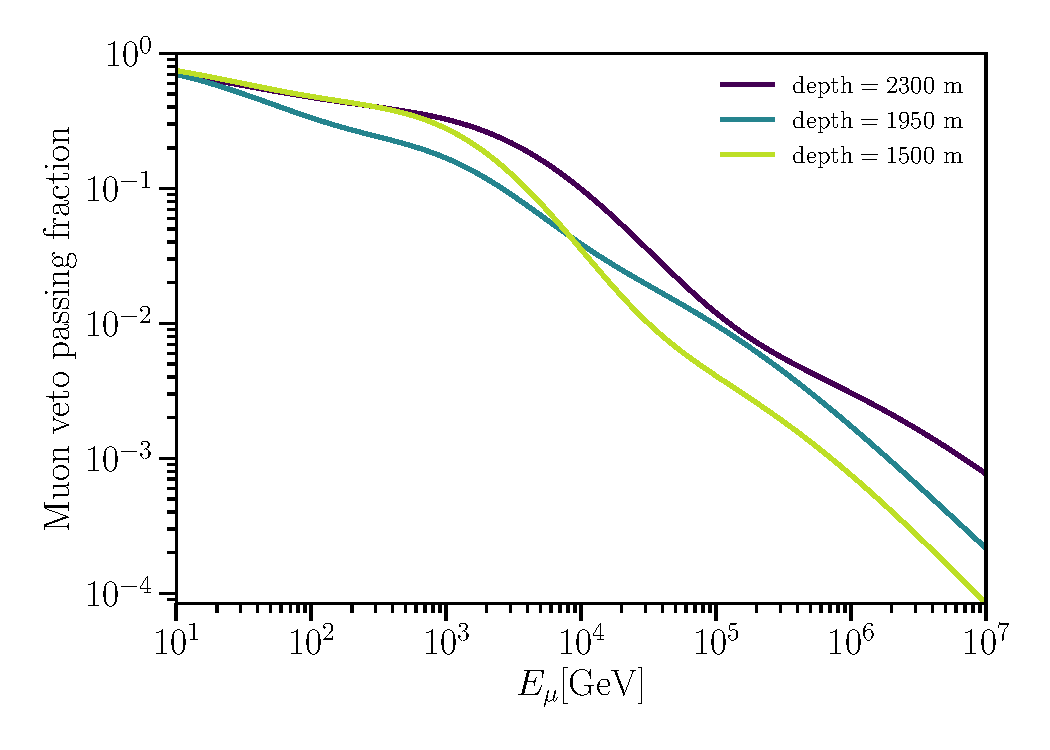
\includegraphics[width=\linewidth]{results/HESE_Final_Paper/figures/plight}
	\internallinenumbers
	\caption{\textbf{\textit{Muon veto passing fraction.}} Each line shows the fraction of muons of a given energy at the detector edge, $E_\mu$, that pass without triggering the veto when entering the detector at a particular depth.
		Three depths are shown: 1500, 1950, and 2300 meters from the surface; with lines of darkening color as the depth increases.
		The veto efficiency increases with the muon energy.
		Differences at various depths are due to the changing ice properties, and varying acceptance as a function of depth due to the asymmetric structure of the veto region.
		At all depths a sigmoid function is fit to the results of muon simulation.
		Above $\sim\SI{100}\TeV$ the passing fraction is extrapolated.}\label{fig:P_light}
\end{figure}

Using the passing fractions in \reffig{fig:P_light} as input and the \nuveto{} code provided in~\cite{Arguelles:2018awr} we calculate the atmospheric passing fraction for each component and flavor using the Hillas-Gaisser H3a~\cite{Gaisser:2013bla,Gaisser:2011cc,Hillas:2006ms} model for the incident cosmic-ray spectra and SIBYLL2.3c~\cite{Riehn:2017mfm} for the hadronic interactions in the air shower.
Using passing fractions derived from alternative cosmic-ray and hadronic interaction models has sub-leading effects in the determination of the astrophysical flux~\cite{Arguelles:2018awr}.
In this work, this was studied by repeating the analysis for different passing fractions that arise from a given combination of cosmic-ray spectrum and hadronic model for a variety of spectra and models that are available in the literature.
We found that the inclusion of these effects in addition to other discrete ice choices mentioned later in \refsec{sec:detector_systematics} increases the reported uncertainty of the astrophysical parameters by at most $\SI{20}\percent$ with respect to errors computed without these effects.
For this reason, these effects are not included in the analysis and are not reflected in the reported errors of any model parameters.
In \reffig{fig:passingfraction} we show the passing fractions for the conventional and prompt neutrino components.
In these figures the left, center, and right panels correspond to $\cos\theta_z$ values of 0.1, 0.3, and 0.9 respectively; the solid lines correspond to muon neutrinos and the dashed lines to electron neutrinos.
From the progression of the panels from left to right, one can see the passing fractions become smaller as one approaches vertical directions.
Vertical muons have the highest probability of reaching the detector, as the overburden they pass through is the smallest.
Though not shown in this figure, the conventional passing fractions differ from neutrinos to anti-neutrinos, see~\cite{Arguelles:2018awr} for details; the appropriate passing fractions are used in this analysis.
\reffigs{fig:conventional_distribution}{fig:prompt_distribution} show the distributions of conventional and prompt neutrinos respectively after this correction is applied.
This reduction in atmospheric background accounts for much of the sensitivity of this analysis to the astrophysical neutrino flux, as the observed down-going atmospheric fluxes in IceCube would otherwise be comparable in magnitude and remain similar in their angular distribution.
This is best seen when comparing the atmospheric fluxes before and after the veto to the measured astrophysical flux as shown in \reffig{fig:neutrino_spectrum}.

% Plot of the passing fraction for different heights (one line per height) (one panel for each costh [3 values])
\begin{figure*}
	\centering
	\subfloat{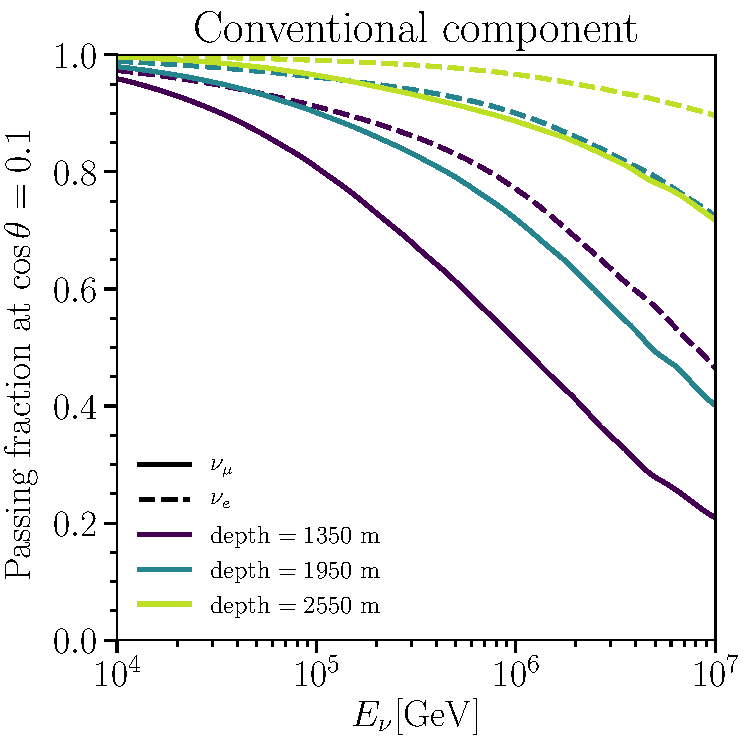
\includegraphics[width=0.3\linewidth]{results/HESE_Final_Paper/figures/conv_0_1_passing_fraction}}
	\subfloat{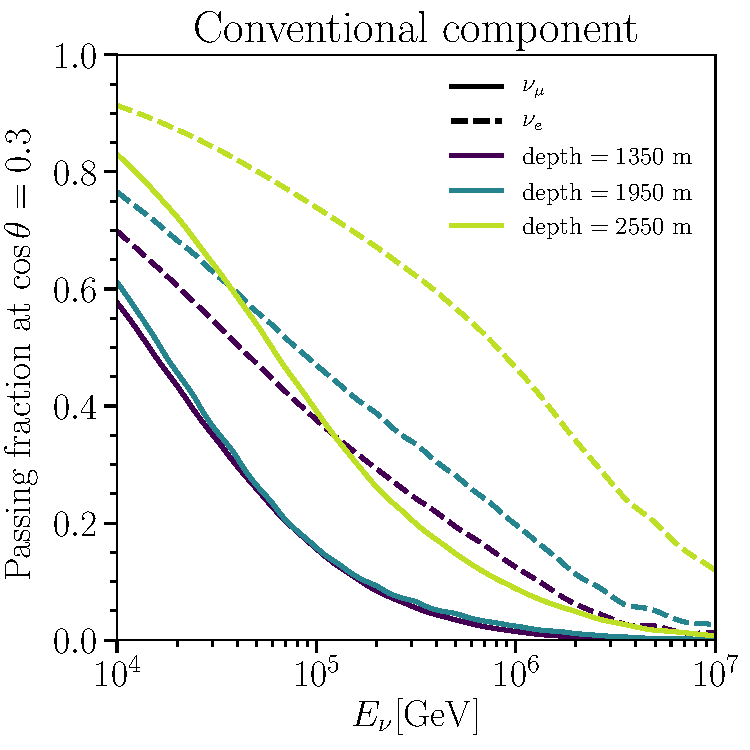
\includegraphics[width=0.3\linewidth]{results/HESE_Final_Paper/figures/conv_0_3_passing_fraction}}
	\subfloat{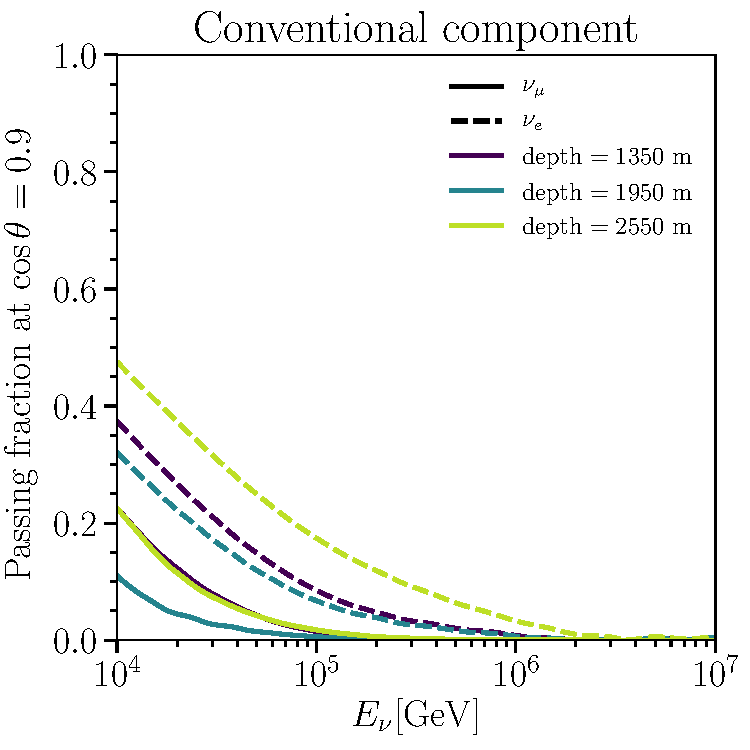
\includegraphics[width=0.3\linewidth]{results/HESE_Final_Paper/figures/conv_0_9_passing_fraction}} \\
	\subfloat{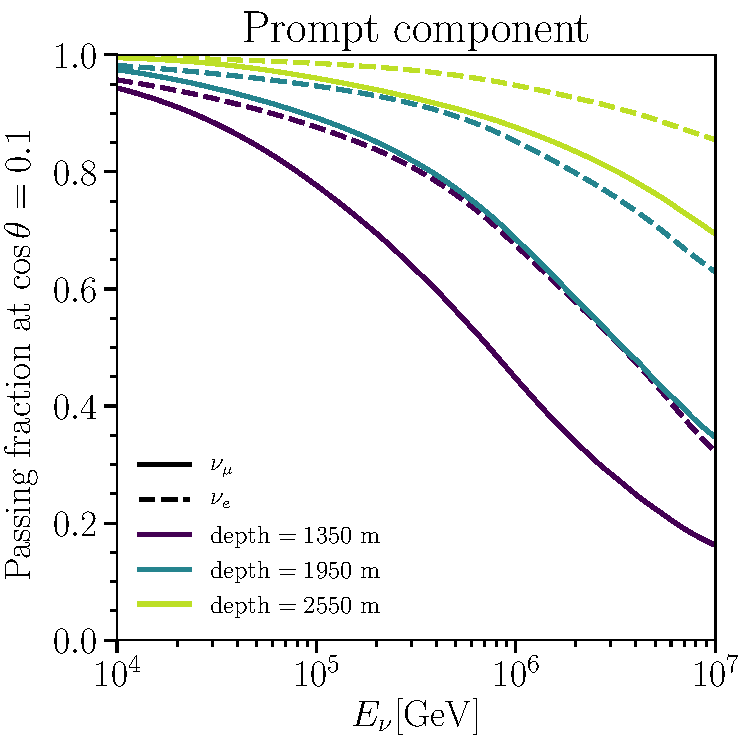
\includegraphics[width=0.3\linewidth]{results/HESE_Final_Paper/figures/prompt_0_1_passing_fraction}}
	\subfloat{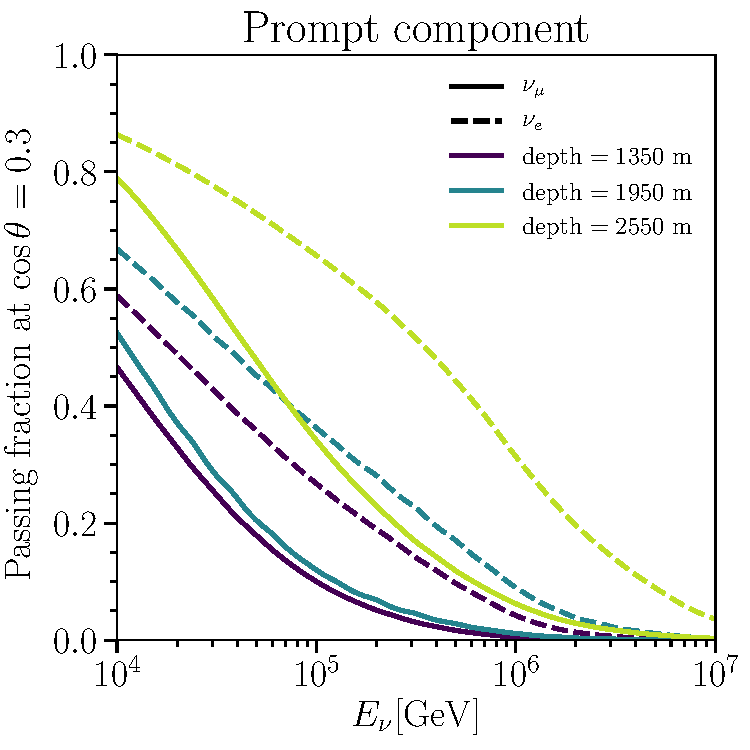
\includegraphics[width=0.3\linewidth]{results/HESE_Final_Paper/figures/prompt_0_3_passing_fraction}}
	\subfloat{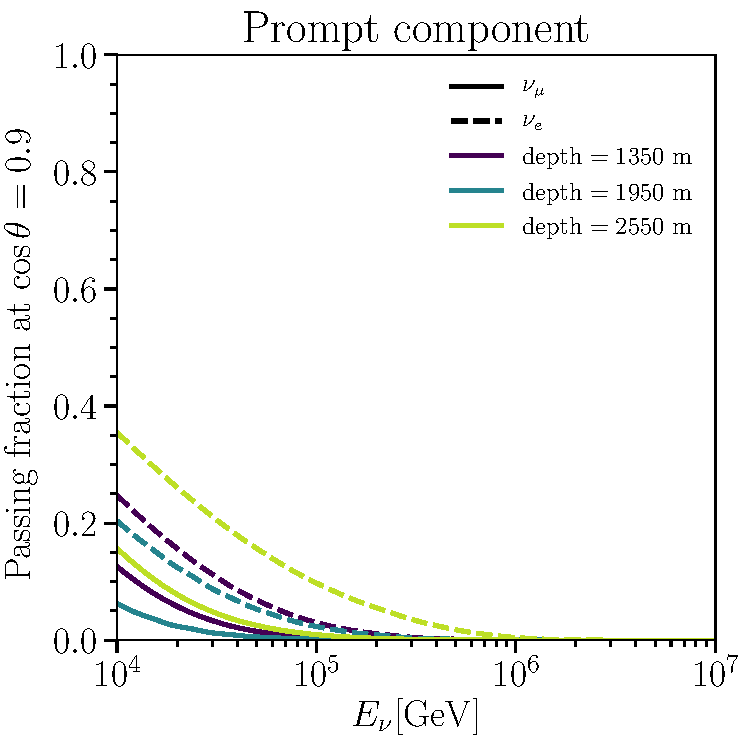
\includegraphics[width=0.3\linewidth]{results/HESE_Final_Paper/figures/prompt_0_9_passing_fraction}}
	\internallinenumbers
	\caption{\textbf{\textit{Conventional and prompt atmospheric component passing fraction.}}
		The top row of plots shows the atmospheric neutrino passing fraction as a function of the neutrino energy for a flux of neutrinos originating from pions and kaons, assuming the Hillas-Gaisser H3a~\cite{Gaisser:2013bla,Gaisser:2011cc,Hillas:2006ms} cosmic-ray model and SIBYLL 2.3c~\cite{Riehn:2017mfm} hadronic interaction model.
		While the bottom row of plots shows the atmospheric neutrino passing fraction for a flux of neutrinos originating from charmed hadrons under the same assumptions.
		Solid lines correspond to muon neutrinos and dashed lines to electron neutrinos.
		The different colors, from darkest to lightest, are for three different detector depths: 1350, 1950, and 2550 meters below the surface.
		The left, center, and right panel correspond to cosine of the zenith angles 0.1, 0.3, and 0.9 respectively (or zenith angles of $\SI{84.3}\degree$, $\SI{72.5}\degree$, and $\SI{25.8}\degree$).}\label{fig:passingfraction}
\end{figure*}

\begin{figure}
	\centering
	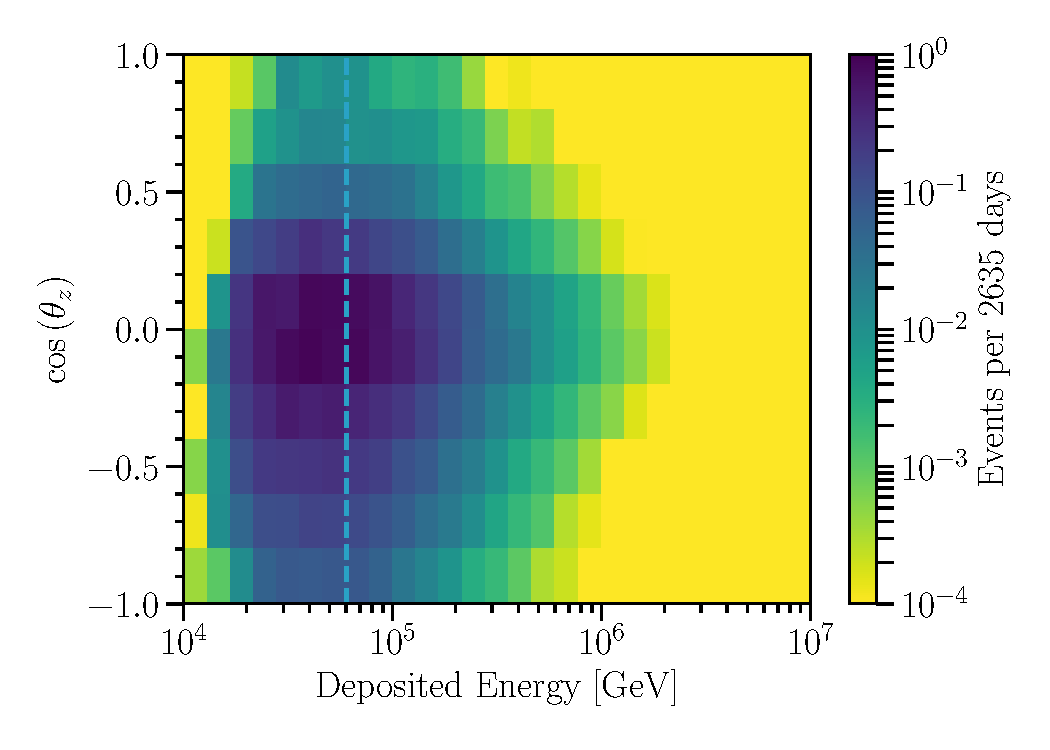
\includegraphics[width=\linewidth]{results/HESE_Final_Paper/figures/diffuse_hist_all_conv}
	\internallinenumbers
	\caption{\textbf{\textit{Expected distribution of atmospheric neutrinos produced by pions and kaons in the sample.}} Distribution of neutrinos that pass the veto as a function of the deposited energy and the cosine of the zenith angle assuming nominal values for the nuisance parameters.
		The dashed line at $\SI{60}\TeV$ marks the low energy cut of the analysis.
		Suppression in the down-going region is due to the veto, while suppression in the up-going region is due to absorption of neutrinos in the Earth.}\label{fig:conventional_distribution}
\end{figure}

\begin{figure}
	\centering
	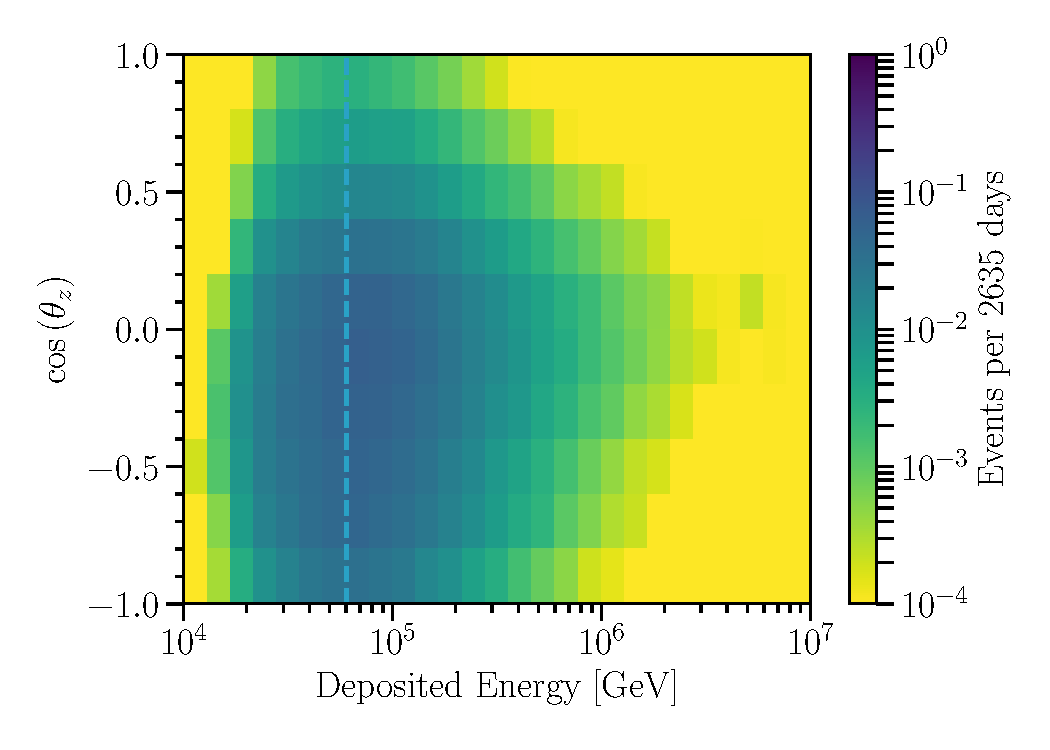
\includegraphics[width=\linewidth]{results/HESE_Final_Paper/figures/diffuse_hist_all_prompt}
	\internallinenumbers
	\caption{\textbf{\textit{Expected distribution of atmospheric neutrinos produced by charmed hadrons in the sample.}} Distribution of neutrinos that pass the veto as a function of the deposited energy and the cosine of the zenith angle assuming nominal nuisance parameters and the BERSS flux calculation for neutrinos from  charmed hadrons~\cite{Bhattacharya:2015jpa}.
		The dashed line at $\SI{60}\TeV$ marks the low energy cut of the analysis.
		Suppression in the down-going region is due to the veto, while suppression in the up-going region is due to absorption of neutrinos in the Earth.}\label{fig:prompt_distribution}
\end{figure}

\begin{figure}
	\centering
	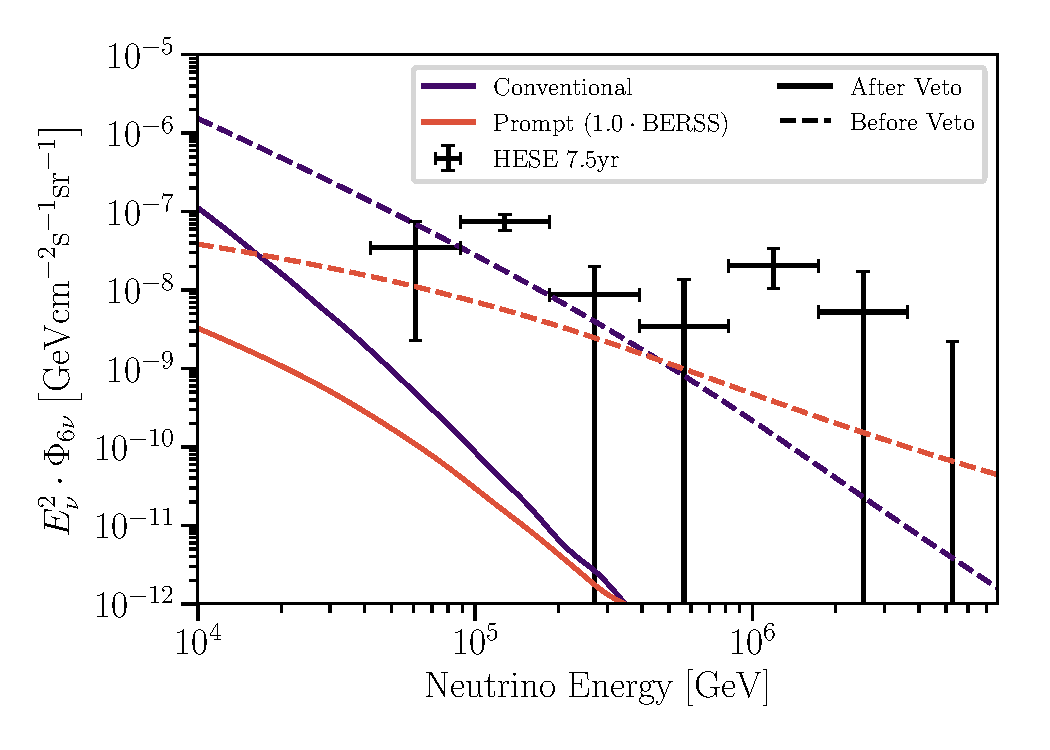
\includegraphics[width=\linewidth]{results/HESE_Final_Paper/figures/neutrino_spectrum}
	\internallinenumbers
	\caption{\textbf{\textit{All-sky astrophysical neutrino flux compared to down-going atmospheric neutrino fluxes before and after the veto.}}
		The atmospheric neutrino fluxes considered in this analysis are shown as dashed lines.
		The solid lines show the product of the atmospheric flux with the passing fraction averaged over depth at a zenith angle of $\SI{0}\degree$.
		The frequentist segmented power-law fit of the all-sky astrophysical flux assuming isotropy as described in \refsec{sec:generic_models} is shown in black.
		This comparison demonstrates the effect of the veto in the down-going region, where it is strongest.
		The suppression of the atmospheric flux becomes weaker towards the horizon, and is not present in the up-going region.
		The dashed lines labelled ``before-veto'' are equivalent to the up-going atmospheric fluxes, with or without the veto, neglecting Earth absorption effects.}
	\label{fig:neutrino_spectrum}
\end{figure}

\subsection{Muon background estimation}
Finally, there is also the possibility of single muons that trigger the event selection without a neutrino interaction in the detector and still pass the veto.
The shape of the atmospheric muon and neutrino fluxes are closely related to each other, and bounded by the cosmic-ray flux so that they must be steeply falling.
The interaction of muons in the atmosphere and ice further softens the muon spectrum from that of cosmic rays.
Although there is uncertainty in the shape of the muon spectrum, the yield of muons from cosmic-ray air showers has more significant modelling uncertainties that stem from uncertainties in the hadronic interaction cross sections~\cite{Pierog:2017nes} and the cosmic-ray composition~\cite{Bluemer:2009zf}.
As we lack the capability to parameterize both the uncertainty in shape and normalization from first principles, we turn to data-driven techniques to constrain the size of this background.
Unfortunately, the data-driven techniques available do not provide us with enough events to determine the shape of the muon background.
For this reason we take a pragmatic approach to treat the muon component.
We use a simulation estimate of the muon flux shape which provides a reasonable estimate for a steeply falling muon spectrum, but neglects shape uncertainties.
The normalization is then constrained using a procedure that tags background muons in data.
The spectrum of atmospheric muons from cosmic-ray air showers is modelled by a parameterization of muons from air showers simulated with the \CORSIKA~\cite{Heck:1998vt} package assuming the Hillas-Gaisser H4a~\cite{Gaisser:2013bla} cosmic-ray flux model and SIBYLL 2.1~\cite{Ahn:2009wx} hadronic model.
A dedicated single muon simulation, called \MUONGUN~\cite{jvsthesis}, is weighted to this flux. 
%Due to the uncertainties in the muon yield of cosmic-ray air showers we use a data-based prior to constrain its normalization and only use the shape from simulation.
To construct the data based prior, a second veto layer inside the original outer veto layer is introduced.
Events that trigger the outer veto layer, but do not trigger this second inner veto layer, are tagged as muons that pass the inner veto.
The muon normalization from simulation is re-scaled from $N_\MUONGUN$ to $2.1\cdot N^\mu_\textmd{tagged}$ to match the number of tagged muons while accounting for the relative size of the fiducial volumes.
Thus, the baseline expected muon flux is given by
\begin{linenomath*}
	\begin{equation}
	\begin{split}
	\frac{d^3\Phi}{d E_\mu d \theta_{z,\mu} d d_\mu} ={}& \frac{d^3\Phi_\texttt{GaisserH4a}}{d E_\mu d \theta_{z,\mu} d d_\mu}(E_\mu, \theta_{z,\mu},d_\mu)\\* & \cdot \frac{2.1 \cdot N^\mu_\textmd{tagged}}{N_\MUONGUN},
	\end{split}
	\label{eq:muon_scaling}
	\end{equation}
\end{linenomath*}
where $\Phi_\texttt{GaisserH4a}$ is the aforementioned parameterization; and $E_\mu$, $\theta_{z,\mu}$, and $d_\mu$ are the muon energy, zenith, and depth at injection respectively.
In \reftab{tbl:tag_muons} we list the number of tagged muons observed per year; in total 17 muons were observed.
The expected distribution of passing atmospheric muon events is shown in \reffig{fig:muons} as a function of the deposited energy and reconstructed cosine of the zenith angle.
The prior on the atmospheric muon rate is chosen to be Gaussian with a $\SI{50}\percent$ standard deviation, this encompasses the statistical uncertainty of our muon background measurement.

\begin{figure}
	\centering
	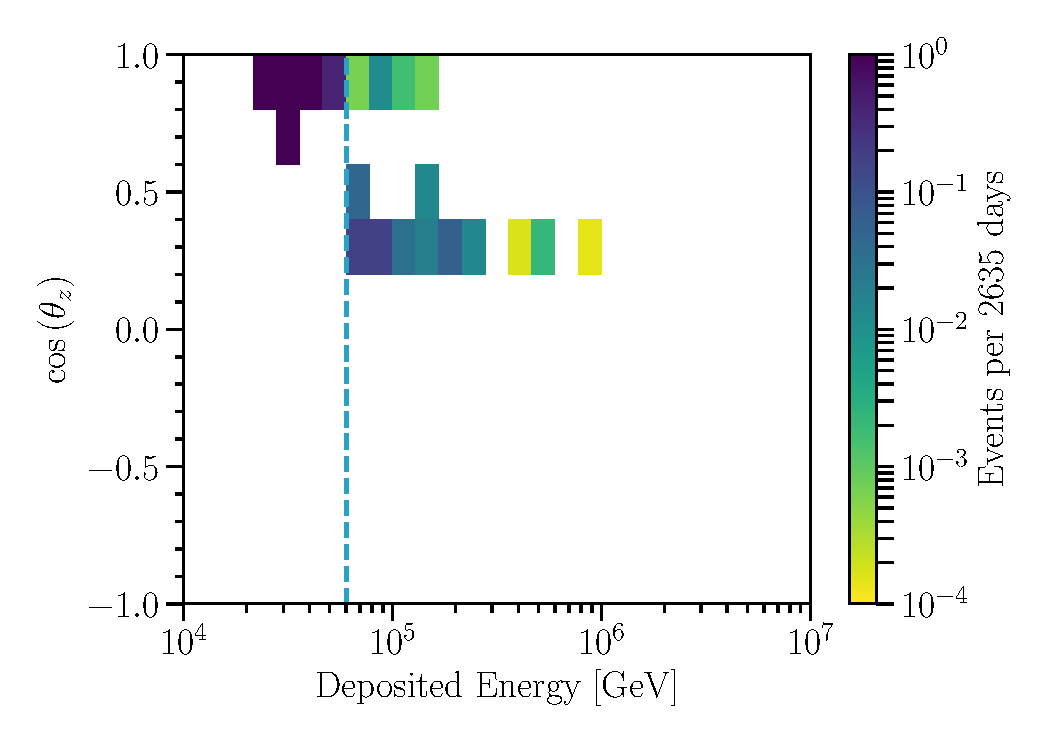
\includegraphics[width=\linewidth]{results/HESE_Final_Paper/figures/diffuse_hist_all_muons}
	\internallinenumbers
	\caption{\textbf{\textit{Expected distribution of atmospheric muons in the sample.}} Distribution of muons that pass the veto as calculated with \MUONGUN~as a function of the deposited energy and the cosine of the zenith angle.
		The normalization is set to match the data driven sub-detector study.
		The dashed line at $\SI{60}\TeV$ marks the low energy cut of the analysis.}\label{fig:muons}
\end{figure}

\begin{table}
	\centering
	% year & number of tagged muons
	\begin{tabular}{l r}
		\toprule
		Season & $N^\mu_{tagged}$ \\
		\midrule
		2010 & 2 \\
		2011 & 1 \\
		2012 & 1 \\
		2013 & 1 \\
		2014 & 2 \\
		2015 & 6 \\
		2016 & 2 \\
		2017 & 2 \\
		\midrule
		Total & 17 \\
		\bottomrule
	\end{tabular}
	\internallinenumbers
	\caption{\textbf{\textit{Number of tagged muons per season.}}
		Table shows the number of tagged muons used to construct the muon normalization prior.
		The first season, 2010, used a partial IceCube configuration with 79 strings, the rest of the seasons took data with the full configuration of 86 strings.
		The larger number of tagged muons in the 2015 season is believed to be a statistical fluctuation.
		The last season, 2017, represents only a partial year of data taking in this paper as the 2017 data processing was not yet completed at the time of this analysis.}\label{tbl:tag_muons}
\end{table}
